% Copyright (C) 2011, 2012 The ScaFaCoS project
%  
% This file is part of ScaFaCoS.
%   
% ScaFaCoS is free software: you can redistribute it and/or modify it
% under the terms of the GNU Lesser Public License as published by the
% Free Software Foundation, either version 3 of the License, or (at your
% option) any later version.
%  
% ScaFaCoS is distributed in the hope that it will be useful, but
% WITHOUT ANY WARRANTY; without even the implied warranty of
% MERCHANTABILITY or FITNESS FOR A PARTICULAR PURPOSE.  See the GNU
% Lesser Public License for more details.
%  
% You should have received a copy of the GNU Lesser Public License
% along with this program.  If not, see <http://www.gnu.org/licenses/>.
%
\documentclass[
paper=a4,                       % paper size
fontsize=11pt,                  % font size
twoside,                        % two sided
footsepline,                    % add a line to separate the footer
headsepline,                    % add a line to separate the header
headinclude=false,              % header does not belong to the text
footinclude=false,              % footer does not belong to the text
pagesize,                       % set the pagesize in a DVI document
bibliography=totocnumbered,     % add the bibliography to the TOC
toc=index,                    % add the index to the TOC
open=right,                      % start a new chapter on the right page
%,DIV12
%,draft
]{scrreprt}

\usepackage[draft]{varioref}    % defines \vref
\usepackage[colorlinks]{hyperref}           % automatically creates links when
                                % using pdflatex, defines \url
\usepackage{ifpdf}              % defines \ifpdf
\usepackage{graphicx}           % handles graphics
\usepackage{makeidx}            % creates the index
\usepackage{color}              % use colors

\usepackage{amssymb}
\usepackage{amsfonts}
\usepackage{amsmath}

\usepackage{calc}               % compute length
\usepackage{ifthen}             % provide ifthen
\usepackage{xspace}
\usepackage[numbers, sectionbib]{natbib}
\usepackage{nicefrac}
\usepackage{longtable}
\usepackage{listings}
\usepackage{tikz}
% \usetikzlibrary{calc,scopes,shapes,fit}
\usepackage{alltt}
\usepackage{paralist}
\usepackage{csquotes}

% \usepackage{pgfplots}
% \pgfplotsset{compat=newest}
% \pgfrealjobname{manual}

%% if pgf/tikz is not installed,
%% comment \usepackage{tikz}, comment \usepackage{pgfplots} and
%% uncomment the following lines
% \long\def\beginpgfgraphicnamed#1#2\endpgfgraphicnamed{%
%   \begingroup
%   \setbox1=\hbox{\includegraphics{figures/#1}}%
%   \openin1=#1.dpth
%   \ifeof1 \box1
%   \else
%     \read1 to\pgfincludeexternalgraphicsdp \closein1
%     \dimen0=\pgfincludeexternalgraphicsdp\relax
%     \hbox{\lower\dimen0 \box1 }%
%   \fi
%   \endgroup
% }

%% This hack enables the inclusion of exported pfg-pictures from subdirectory ./figures/.
%% Use a command like 'pdflatex -shell-escape --jobname p2nfft_ewald_split manual.tex'
%% to externalize graphics and move them into directory ./figures/.
%% Uncomment the following line before 'svn ci':
\def\enablemypgfhack{1}
\long\def\beginmypgfhack#1#2\endmypgfhack{%
  \ifx\enablemypgfhack\undefined
    \beginpgfgraphicnamed{#1}#2\endpgfgraphicnamed
  \else
    \includegraphics{figures/#1}
  \fi
}


% For building the distribution docs, disable todo boxes.
%\usepackage[disable]{todonotes}
\usepackage{todonotes}

\usepackage{placeins}

\renewcommand{\topfraction}{0.85}
\renewcommand{\textfraction}{0.1}
\renewcommand{\floatpagefraction}{0.75}

% required so that we can set index numbers bold
% \index{Some example|main}
\newcommand*{\main}[1]{\textbf{\hyperpage{#1}}}
\newcommand*{\mainul}[1]{\underline{\textbf{\hyperpage{#1}}}}

%%%%%%%%%%%%%%%%%%%%%%%%%%%%%%%%%%%%%%%%%%%%%%%%%%
%%%%%%%%% New Commands and Environments %%%%%%%%%%
%%%%%%%%%%%%%%%%%%%%%%%%%%%%%%%%%%%%%%%%%%%%%%%%%%
\newcommand{\fcs}{\mbox{\textsf{ScaFaCoS}}\xspace}
\newcommand{\ie}{\textit{i.e.}\xspace}
\newcommand{\eg}{\textit{e.g.}\xspace}
\newcommand{\etal}{\textit{et al.}\xspace}

\newcommand{\solvertoindex}[1]{
  \index{#1|main}
  \index{Solver!#1|main}
}

\newcommand{\functiontoindex}[1]{
  \index{Functions!#1|main}
}

\newcommand{\ufunctiontoindex}[1]{
  \index{Functions!#1|mainul}
}


\newcommand{\N}{\ensuremath{\mathbb{N}}}
\newcommand{\T}{\ensuremath{\mathbb{T}}}
\renewcommand{\S}{\ensuremath{\mathbb{S}}}
\newcommand{\NZ}{\ensuremath{\mathbb{N}_{0}}}
\newcommand{\Z}{\ensuremath{\mathbb{Z}}}
\newcommand{\Q}{\ensuremath{\mathbb{Q}}}
\newcommand{\R}{\ensuremath{\mathbb{R}}}
\newcommand{\C}{\ensuremath{\mathbb{C}}}
\newcommand{\cO}{{\cal O}}
\newcommand{\cK}{{\cal K}}

\newcommand{\e}{\mbox{\rm{e}}}
\newcommand{\im}{\mbox{\scriptsize\rm{i}}}
\newcommand{\eip}[1]{\e^{+2\pi\im #1}}
\newcommand{\eim}[1]{\e^{-2\pi\im #1}}
\newcommand{\adj}{{\vdash \hspace*{-1.72mm} \dashv}}


\makeindex
\begin{document}

%% LOGO
% For a logo to come
% \titlehead{
%   \begin{center}
%     \includegraphics[width=5cm]{logo/transparentbg}
%   \end{center}
% }

%\subject{}
\title{\fcs Manual}
\author{}
\date{\today}
\maketitle

\setcounter{tocdepth}{1}
\tableofcontents
\pdfbookmark{Contents}{toc}

\listoftodos
\pdfbookmark{Todo List}{todo}

\part{User's Guide}
\chapter{Introduction}
\label{cha:introduction}

\todo[inline]{Fix introduction}

\section{What ScaFaCoS Computes}

\subsection{Fully Non-Periodic Boundary Conditions}
In this part we apply our fast summation algorithm to a system
of $M$ charged particles located at source nodes $\mathbf x_l\in \R^3$ with charge $q_l\in\R$.
We are interested in the evaluation of the electrostatic potential $\phi$ at target node $\mathbf x_j\in \R^3$,
\begin{equation}\label{eq:potential_0dp}
 \phi (\mathbf x_j) = \underset{l \neq j}{\sum_{l=1}^{M}} \dfrac{q_l}{\left\| \mathbf x_j - \mathbf x_l \right\|_2},
 \quad j=1,\hdots,M,
\end{equation}
and the electrostatic fields $\mathbf E$ evaluated at position $\mathbf x_j\in \R^3$,
\begin{equation}\label{eq:fields_0dp}
   \mathbf E(\mathbf x_j)
   = - \underset{l\neq j}{\sum_{l=1}^{M}} q_l \frac{\mathbf x_j - \mathbf x_l}{\|\mathbf x_j - \mathbf x_l \|_2^3},
   \quad j=1,\hdots,M.
\end{equation}
Furthermore we are interested in the computation of the total electrostatic potential energy
\begin{equation*}
  U := \frac{1}{2} \sum\limits_{j = 1}^{M} q_j \phi(\mathbf x_j),
\end{equation*}
which can be evaluated straightforward after the computation of the potentials $\phi(\mathbf x_j), j=1,\hdots,M$.
\todo{Virial}

\subsection{Fully Periodic Systems}
We consider a system of charged particles coupled via the Coulomb potential, a cubic simulation box with
edge length $B$, containing $M$ charged particles, each with a charge $q_l\in\R$, located at $\mathbf x_l\in [0,B)^3$.
Periodic boundary conditions in a system without cut-off is represented by replicating the simulation
box in all directions of space.
The electrostatic potential $\phi$ at $\mathbf y\in [0,B)^3$, can be written as a lattice sum,
see \cite[Chapter 12]{FrSm02} and \cite{Sut06},
\begin{equation}\label{eq:potential_3dp}
  \phi(\mathbf x_j)
  = \sum_{\mathbf r\in \mathbb Z^3} \underset{ l\neq j \,{\rm for}\, \mathbf r= \mathbf 0}{\sum_{l=1}^M}
    \frac{q_l}{\|\mathbf x_j -\mathbf x_l +\mathbf r B\|_2}\,,
    \quad j=1,\hdots,M
\end{equation}
and the electrostatic field $\mathbf E$ evaluated at position $\mathbf x_j\in [0,B)^3$ is given by
\begin{equation}\label{eq:fields_3dp}
  \mathbf E(\mathbf x_j)
  = - \sum_{\mathbf r\in \mathbb Z^3}
    \underset{ l\neq j \,{\rm for}\, \mathbf r= \mathbf 0}{\sum_{l=1}^M}
    q_l \frac{\mathbf x_j -\mathbf x_l +\mathbf r B}{\|\mathbf x_j -\mathbf x_l +\mathbf r B \|_2^3},
    \quad j=1,\hdots,M\, ,
\end{equation}
Furthermore we are interested in the computation of the total electrostatic potential energy
\begin{equation*}
  U := \frac{1}{2} \sum\limits_{j = 1}^{M} q_j \phi(\mathbf x_j),
\end{equation*}
which can be evaluated straightforward after the computation
of the potentials $\phi(\mathbf x_j)$, $j=1,\hdots,M$ like in the non-periodic case.
\todo{Virial}




\section{Acknowledgements}

This is a network project of German research groups working on a
unified parallel library for various methods to solve electrostatic
(and gravitational) problems in large particle simulations. The
project is financed by the German Ministry of Education and Science
(BMBF) under contract number 01 IH 08001 A-D.  Main focus of the
project is to provide methods for electrostatic problems and to
implement efficient parallel methods in order to scale up to thousands
of processors.  \fcs is supported within the period 01/01/2009 -
31/12/2011.


\section{Licensing}

This library is open source software.  It comes with parts that are
distributed under the GNU General Public License (GPL) and parts that
are distributed under the GNU Lesser General Public License (LGPL).
Please refer to the documentation of the individual solver methods for
details.  The toplevel configure script provides a switch
\texttt{--disable-gpl} to disable the build of all methods which allow
only a distribution under the GPL.


\section{Requirements}
\label{sec:requirements}
\index{requirements|main}

The following libraries and tools are required to be able to compile
and use \fcs:

\begin{description}
\item[MPI] \index{MPI} As \fcs is parallel software, you will need a
  working MPI environment that implements at least the MPI standard
  version 1.2.
  \todo{Is MPI 1.2 really enough?}
\item[C99 compiler] \index{C99} The C-code of \fcs uses the C99
  standard, therefore a compiler that is able to compile C99 code must
  be available. We do not know of any recent platform that does not
  provide a C99 compiler.
\item[C++ compiler] \index{C++} Some methods (\eg VMG) require a C++
  compiler.
\item[Fortran 2003 compiler] \index{Fortran 2003} The Fortran code of
  some methods (\eg FMM) does require a Fortran 2003 compiler.
\item[FFTW] \index{FFTW} Some solver methods (\eg P$^3$M and P2NFFT)
  need the FFTW library version 3.3.0 or later
  \footnote{\url{http://www.fftw.org/}} for Fourier transforms.  For
  P2NFFT, the MPI interface of FFTW3 has to be available. You do
  not only need the library itself, but also the header files.
  Depending on the operating system, these may come in separate
  development packages (\eg \texttt{fftw3-dev}).
  \todo{FFTW3 is part of the library}
\end{description}

\section{Feature Matrix}
\label{sec:feature_matrix}
\index{feature matrix|main}

  \begin{table}[htbp]
    \begin{minipage}{\textwidth}
      \centering
      \begin{tabular}{|l||*{10}{c|}}
        \hline
        &
        \rotatebox{90}{\textbf{FMM}} &
        \rotatebox{90}{\textbf{MEMD}} &
        \rotatebox{90}{\textbf{MMM*D}} &
        \rotatebox{90}{\textbf{P2NFFT}} &
        \rotatebox{90}{\textbf{P3M}} &
        \rotatebox{90}{\textbf{PEPC}} &
        \rotatebox{90}{\textbf{PP3MG}} &
        \rotatebox{90}{\textbf{VMG}} &
        \rotatebox{90}{\textbf{Direct}} &
        \rotatebox{90}{\textbf{Ewald}}
        \\
        \hline
        \hline

        \textbf{3D-periodic} &
        + & + & -- & + & + & +                                     & +        & + & + & + \\
        \hspace{2em}\textbf{non-cubic, cuboid} &
        -- & -- &   & + & + & +\footnote{untested}                 & +        & ? & + & + \\
        \hspace{2em}\textbf{non-cubic, non-cuboid} &
        ? & ? &   & -- & ? & +\footnote{untested}                   & ?        & ? & ? & ? \\
        \hspace{2em}\textbf{Virials} &
        ? & -- &   & ?\footnote{diagonal approximation} & ? & --\footnote{implementation planned}   & (scalar) & ? & ? & -- \\
        \hline

        \textbf{Nonperiodic} &
        + & -- & -- & + & -- & +                                   & --        & ? & + & -- \\
        \hspace{2em}\textbf{non-cubic} &
        -- &   &   & --\footnote{implementation planned} &   & +                                     &          & ? & + &   \\
        \hspace{2em}\textbf{Virials} &
        + &   &   & + &   & --\footnote{implementation planned}    &          & ? & + &   \\
        \hline

        \textbf{Partially periodic} &
        + & -- & + & --\footnote{implementation planned} & -- & +\footnote{untested}                & --        & ? & + & -- \\
        \hline

        \textbf{Tunable accuracy} &
        + & -- & + & + & + & --                                    & --        & -- & -- & + \\
        \hline

        \textbf{Delegate near-field} &
        -- & -- & ? & + & + & --                                   & ?        & ? & -- & -- \\
        \hline

      \end{tabular}
    \end{minipage}
    \caption{Overview of the features of the different solvers.}
  \end{table}
%%% Local Variables: 
%%% mode: latex
%%% TeX-master: ug.tex
%%% End: 


\chapter{Compling and installing \fcs}
\label{cha:compiling}

\index{Compilation}
\index{Installation}
\index{SVN}

\todo[inline]{\LaTeX this code}
\begin{verbatim}
0) If you are building the code from the SVN tree, read README-SVN first.

1) Compile:
   a) Run './configure' with suitable options.  See below for common setups.
      You can pass '--enable-fcs-solvers=...' to enable all or only some solvers.
      You can pass '--disable-fcs-SOLVER' to disable a particular solver, e.g.,
      '--disable-fcs-vmg'.
      You can have build trees separate from the source tree, e.g.:
        mkdir ../build-debug
        cd ../build-debug
        ../scafacos_fcs/configure -C CFLAGS=-g FCFLAGS=-g [...]
      See './configure --help' and './configure --help=recursive' for all
      supported options.
      The -C aka. --config-cache option greatly speeds up configuring all the
      subdirectories.
   b) Run 'make'.  Parallel make should work.

2) run test-programs:
   a) Run 'make check'.  This tries to be smart about finding out how to
      start MPI jobs on your system.  If the chosen method is wrong, you
      might have to edit test/defs.in and/or rerun configure with an argument
      of MPIEXEC=... set to the MPI invocation program on your system.

If that doesn't work, then you can alternatively do the following:

   b_1) cd test/c (if you are a c-programmer) or
   b_2) cd test/fortran (if you intend to use fortran)
   c) choose a method you want to run
   d) $mpi_call_on_my_machine ./test_$method ../inp_data/$method/$method_conf.in

3) Sources of the fcs-interface are located in $INSTALL_DIR/src

4) Sources of the ScaFaCos methods can be found in INSTALL_DIR/lib

5) Optionally run 'make install' to install the library and header files.

6) To find out compiler and linker flags to use in packages linking against FCS,
   you can use
      pkg-config --cflags scafacos-fcs
      pkg-config --libs scafacos-fcs

   if you have the pkg-config package installed.

Configure setups for common systems
===================================

Generally, if you set both MPICC and CC, or MPICXX and CXX, or MPIFC and FC,
you may need to ensure that compatible compiler drivers are used.

You may want to add -C to cache configure test results; this speeds up the
recursive configure scripts.

GNU/Linux
---------
It should work to use one of

  ./configure
  ./configure FCFLAGS=-fno-underscoring

depending on which ABI you need to maintain with respect to other Fortran code.
If you are using gfortran, you need version 4.3 or newer for Fortran 2003 support.


BlueGene
--------
The following alternative configurations should work (the --build and --host
arguments ensure configure enables cross-compilation mode):

  ./configure --build=powerpc64-bgp-linux-gnu --host=powerpc-ibm-linux \
     MPICC=mpixlc_r MPIFC=mpixlf2003_r MPICXX=mpixlcxx_r CFLAGS='-qfullpath -O2' \
     FCFLAGS='-qfullpath -qarch=450 -qtune=450 -qxlf2003=nostopexcept -O3 -qipa -qipa=inline=key2addr'

  ./configure --build=powerpc64-bgp-linux-gnu --host=powerpc-ibm-linux \
     MPICC=mpixlc_r MPIFC=mpixlf2003_r MPICXX=mpixlcxx_r \
     CFLAGS='-g -qfullpath -qdbxextra -qcheck' FCFLAGS='-g -qfullpath'

  ./configure --build=powerpc64-bgp-linux-gnu --host=powerpc-ibm-linux \
     MPICC=mpixlc_r MPICXX=mpixlcxx_r MPIFC=mpixlf2003_r \
     CPPFLAGS='-I/bgsys/drivers/ppcfloor/comm/include -I/bgsys/drivers/ppcfloor/arch/include' \
     CFLAGS='-O3 -g -qmaxmem=-1 -qarch=450 -qtune=450' \
     FCFLAGS='-O3 -g -qmaxmem=-1 -I/bgsys/drivers/ppcfloor/include -qarch=450 -qtune=450' \
     LDFLAGS='-L/bgsys/drivers/ppcfloor/lib -L/bgsys/local/lapack/lib -L/bgsys/local/lib' \
     BLAS_LIBS='-lesslbg -lxlf90_r'

Juropa
------

Building with the Intel compiler suite should work:

  ./configure MPICC=mpicc MPICXX=mpicxx MPIFC=mpif90
\end{verbatim}
%%% Local Variables: 
%%% mode: latex
%%% TeX-master: ug.tex
%%% End: 

\chapter{Interface}
\label{cha:interface}
\raggedbottom
\renewcommand\arraystretch{1.75}

%%% Local Variables: 
%%% mode: latex
%%% TeX-master: ug.tex
%%% End: 



\section{Basic Ideas of the Interface}

The basic idea of the ScaFaCoS interface is that it should be very simple to include the library to existing programs and packages.
Therefore the aim was to have as few required functions as possible for adding the library. To use the library one has only five functions
to add to an existing code, if the default parameters for each solver suffice. Of course there is the possibility to change the
parameters of the solvers by use of additional functions. In this sections the basic functions will be described, so that the reader
is able to add the ScaFaCoS library to his or her own code. \\
To understand the following sections, one has to know the idea behind the use of the library. One usage cycle is divided into five
sections, which are mapped to the five required functions. These sections are:
\begin{enumerate}
  \item Initialization of the library
  \item Setting the non-solver specific parameters
  \item Tuning the solver
  \item Running the solver (more then once if needed)
  \item Destroying allocated resources of the library
\end{enumerate}
These five steps are each tied to one call of the respective function. In the initialization step the communicator used by the library is
defined, as well as the solver to used is chosen. During the second step the global parameters like system size and periodicity of the
system are set. Within the third step solver-specific tuning methods are called (where possible) which try to utilize the system
in order to improve the solvers performance or set up data structures requiring knowledge about particle positions. The central step is
the fourth step in which the calculation of the Coulomb interactions takes place. E.g. within a MD code this step can be called for
each time step, in order to take into consideration the shifting particle positions. After the calculation is or calculations are done,
the last step frees all the resources which were used by the library.\\
The interface functions are provided in a (C++ compatible) C version and in a Fortran version, which is a wrapper of the C version. In
the section both variants will be described. Table \ref{tab:solver_overview} gives an overview about all solvers included until the
creation of this documentation.

\begin{table}[tbp]
\begin{center}
\begin{tabular}{|c|p{0.55\textwidth}|}
\hline
  ScaFaCoS abbreviation         &    full solver name     \\
\hline
\hline
  direct                        &    Direct solver (\ref{cha:direct})       \\
\hline
  ewald                         &    Ewald summation (\ref{cha:ewald})              \\
\hline
  fmm                           &    Fast Multipole Method (\ref{cha:fmm}) \\
\hline
  memd                          &    Maxwell equations Molecular Dynamics (\ref{cha:memd})\\
\hline
  mmm1d                         &    (\ref{cha:mmm1d})\\
\hline
  mmm2d                         &    (\ref{cha:mmm2d})\\
\hline
  pepc                          &    Pretty Efficient Parallel Coulomb solver (Barnes-Hut Tree Code) (\ref{cha:pepc})\\
\hline
  pp3mg                         &    Particle-Particle Particle-Multigrid solver (\ref{cha:pp3mg}) \\
\hline
  p2nfft                        &    Parallel Particle Non-Equidistant FFT solver (\ref{cha:p2nfft})\\
\hline
  p3m                           &    Particle-Particle Particle-Mesh method (\ref{cha:p3m})\\
\hline
  vmg                           &    Versatile Multigrid method (\ref{cha:vmg})\\
\hline
\end{tabular}
\end{center}
\caption{Solvers implemented in ScaFaCoS (02/2012)}
\label{tab:solver_overview}
\end{table}

\section{Use of the ScaFaCoS Library}

In this section the implementation of the steps presented in the previous section will be explained. Before the actual implementation
of the ScaFaCoS library to a code will be described, the headers and modules and the data types and constants provided by the library
will be presented.

\subsection{Header and Modules}
To simplify the inclusion of the library into existing or newly written codes, the library provides either a single header for C or a
single module for Fortran which needs to be included into the code. For C this is the \textit{fcs.h} header and for Fortran this is the
module \textit{fcs\_module} (fig. \ref {fig:header_module}). 

\begin{figure}[htb]
\begin{lstlisting}[language=C, frame=trBL]
/* inclusion in C */
#include "fcs.h"
\end{lstlisting}
\begin{lstlisting}[language=Fortran, frame=trBL]
! inclusion in Fortran
use fcs_module
\end{lstlisting}
\caption{Use of the provided header / module of the ScaFaCoS library.}
\label{fig:header_module}
\end{figure}

Due to the use of the pkg-package tool \cite{pkg-package}, there is a easy way to get the correct library and include options for the compilation
of the code with ScaFaCoS included. Figure \ref{fig:pkg-usage} shows how pkg-config can be used to that end at an example. In order to use pkg-config
\textit{make check} has to be used before so that an installation is created.

\begin{figure}[htb]
\begin{lstlisting}[language=bash, breaklines, prebreak={\raisebox{0ex}[0ex][0ex]{\ensuremath{\hookleftarrow}}} ]
export PKG_CONFIG_PATH=<ScaFaCoS install path>/lib/pkg-config:${PKG_CONFIG_PATH}
FCSLIB=$(shell pkg-config --libs scafacos-fcs)
FCSINC=$(shell pkg-config --cflags scafacos-fcs)
gcc -o <application name> [other options] ${FCSLIB} ${FCSINC} <source(s)>
\end{lstlisting}
\caption{exemplary usage of pkg-config to get the necessary information for compilation}
\label{fig:pkg-usage}
\end{figure}


\subsection{Data Types and Constants}
\solvertoindex{data types}
The library provides data types for C (table \ref{tab:c_data_types}) and data kinds Fortran (table \ref{tab:fortran_data_kinds}), which are either defined within the configure script or set to default values by the
configure script. During this procedure the Fortran data types are matched to the corresponding C data types in order to ensure
compatibility between the Fortran wrapper and the C functions underneath. The default values for these data types are:


\begin{table}[tbp]
\begin{center}
\begin{tabular}{|c|c|}
\hline
  ScaFaCoS data type            &    data type (C)     \\
\hline
  fcs\_int                      &    int        \\
\hline
  fcs\_float                    &    double        \\
\hline
\end{tabular}
\end{center}
\caption{ScaFaCoS data types for C}
\label{tab:c_data_types}
\end{table}

\begin{table}
\begin{center}
\begin{tabular}{|l|l|}
\hline
  ScaFaCoS data type              &    data type (Fortran 2003)     \\
\hline
\hline
  fcs\_integer\_kind\_isoc        &    C\_INT                \\
\hline
  fcs\_real\_kind\_isoc           &    C\_DOUBLE            \\
\hline
\end{tabular}
\end{center}
\caption{ScaFaCoS data kinds for Fortran}
\label{tab:fortran_data_kinds}
\end{table}

In addition to that the library supplies an additional data type, which is used for data 
transport between the different functions. This data type is FCS, which is a pointer to a struct
containing the common information about the simulation system (box size, periodicity, ...).
From the user side it is only used as an argument to the different library functions
and must not be changed by him. Otherwise the behavior of the library is undefined.\\
Furthermore there are some definitions, which are used within the library and which can 
be used by the user.

\begin{table}
    \begin{center}
    \begin{tabular}{|l|r@{\,=\,}l|}
        \hline
        C macro name                    &               \multicolumn{2}{c}{value}                     \\
        \hline
        \hline
        FCS\_E                          &               Euler constant $e$         & $2.71828\hdots$  \\
        \hline
        FCS\_LOG2E                      &               $\log_2e$                  & $1.44269\hdots$  \\
        \hline
        FCS\_LOG10E                     &               $\log_{10}e$               & $0.43429\hdots$  \\
        \hline
        FCS\_LN2                        &               $\log_e2$                  & $0.69314\hdots$  \\
        \hline
        FCS\_LN10                       &               $\log_e10$                 & $2.30258\hdots$  \\
        \hline
        FCS\_PI                         &               $\pi$                      & $3.14159\hdots$  \\
        \hline
        FCS\_PI\_2                      &               $\nicefrac{\pi}{2}$        & $1.57079\hdots$  \\
        \hline
        FCS\_PI\_4                      &               $\nicefrac{\pi}{4}$        & $0.78539\hdots$  \\
        \hline
        FCS\_1\_PI                      &               $\nicefrac{1}{\pi}$        & $0.31830\hdots$  \\
        \hline
        FCS\_2\_PI                      &               $\nicefrac{2}{\pi}$        & $0.63661\hdots$  \\
        \hline
        FCS\_2\_SQRTPI                  &               $\nicefrac{1}{\sqrt{\pi}}$ & $0.31830\hdots$  \\
        \hline
        FCS\_SQRT2                      &               $\sqrt{2}$                 & $1.41421\hdots$  \\
        \hline
        FCS\_SQRT1\_2                   &               $\nicefrac{1}{\sqrt{2}}$   & $0.70710\hdots$  \\
        \hline
    \end{tabular}
    \end{center}
    \caption{ScaFaCoS mathematical macros}
    \label{tab:c_macros_mathematical}
\end{table}

The mathematical constants (table \ref{tab:c_macros_mathematical}) can be used in C and in Fortran. Due to the \textit{FCS\_} prefix it
is ensured, that they don't interfere with eventual definitions by the user or the system for these values. As a mean to simplify
error handling within the library the error values are also defined as macros (table \ref{tab:c_macros_error}).

\begin{table}
    \begin{center}
    \begin{tabular}{|l|p{0.55\textwidth}|}
        \hline
        C macro name                    &               meaning                                 \\
        \hline
        \hline
        FCS\_SUCCESS                    &       no error occurred (deprecated)                   \\
        \hline
        FCS\_NULL\_ARGUMENT             &       an argument passed to the method was undefined  \\
        \hline
        FCS\_ALLOC\_FAILED              &       an internal allocation of memory failed         \\
        \hline
        FCS\_WRONG\_ARGUMENT            &       it was tried to set an parameter belonging to
                                                another method                                  \\
        \hline
        FCS\_MISSING\_ELEMENT           &       a system parameter was not set                  \\
        \hline
        FCS\_LOGICAL\_ERROR             &       a violation of set parameters was encountered   \\
        \hline
        FCS\_INCOMPATIBLE\_METHOD       &       the method cannot be used for given system      \\
        \hline
        FCS\_MPI\_ERROR                 &       an MPI error was encountered                    \\
        \hline
        FCS\_FORTRAN\_CALL\_ERROR       &       an error occurred while using the Fortran wrapper\\
        \hline
    \end{tabular}
    \end{center}
    \caption{ScaFaCoS error values}
    \label{tab:c_macros_error}
\end{table}

Furthermore there are two structures defined, which are used internally to store provided parameters and
error details. These structures are called \textit{FCS} and \textit{FCSResult}. \textit{FCS} will be created
during the initialization step (\ref{sec:init_step}) and filled during the parameter setup step (\ref{sec:par_setup}).
After that it needs to be supplied for the tuning (\ref{sec:tune_step}) and calculation step (\ref{sec:run_step}).
Finally it will be freed during the clean up step (\ref{sec:clean_up_step}). \textit{FCSResult} will be
used for error handling and the needed getter-functions will be explained in the
section on error handling (\ref{sec:error_handling}) 

\subsection{Initialization Step}
\label{sec:init_step}
\functiontoindex{fcs\_init}
During the initialization step, the library is supplied with all information that cannot be changed during
the simulation by use of the function \textit{fcs\_init} (fig. \ref{fig:fcs_init}). This information includes 
the MPI communicator, which is to be used and the chosen method.
With this information a \textit{FCS} data structure is created. The calls in C and Fortran differ only in
the data types of the arguments. While C supplies an unique MPI\_Comm type for MPI communicators, in Fortran
these are represented by integer values. Also Fortran does not grant access to pointers in the same fashion
as C does. In order to circumvent this, the Fortran interface uses the c\_ptr type (\cite[p. 565f.]{fortran-handbook})
as a replacement.



The initialization step is mandatory for the use of the ScaFaCoS library, since in it the most important information is
set. This is on the one hand the choice of solver and on the other hand the parallel environment in which the library
is used, as described by the MPI communicator. (see also table \ref{tab:fcs_init_parameters})\\
If the function returns successfully, it returns a \textit{NULL} value, else it returns as an error value \textit{FCS\_NULL\_ARGUMENT} if one
of the provided arguments is not defined or \newline\textit{FCS\_ALLOC\_FAILED} if the \textit{FCS} structure could not be allocated.
If an invalid solver was chosen, then the function returns \textit{FCS\_WRONG\_ARGUMENT}, e.g. if a method was chosen, that
was disabled in the configure script.

\begin{table}
\begin{center}
\begin{tabular}{|p{0.12\textwidth}|p{0.35\textwidth}|p{0.45\textwidth}|}
          \hline
          parameter name        &       description                                         &   valid values                        \\
          \hline
          \hline
          handle                &       pointer to parameter containing structure           &   FCS (C) or type (c\_ptr) (Fortran)   \\
          \hline
          method                &       chosen method                                       &   abbreviation from table \ref{tab:solver_overview} \\
          \hline
          comm                  &       MPI communicator the library has to work on         &   valid MPI communicator              \\
          \hline 
\end{tabular}
\end{center}
\caption{Parameters for fcs\_init}
\label{tab:fcs_init_parameters}
\end{table}

\subsection{Parameter Setup Step}
\label{sec:par_setup}
\functiontoindex{fcs\_common\_set}
This step is two-fold, the parameters describing the system are set, as well as the parameters for the solver
chosen in the initialization step (\ref{sec:init_step}). The former is mandatory, because the information about
the system is needed by the solvers in order to calculate the correct forces, while the latter is optional as
the solvers provide (non-optimal) default parameters for themselves.

As can be seen in figure \ref{fig:fcs_set_common} the calls differ for C and Fortran. Since plain C does not provide a logical data type, e.g. bool,
the C interface uses integer variables for this purpose. The Fortran data kinds are linked to the C data types set in the configure script. Possible
return values are \textit{NULL} for a successful return and either \newline\textit{FCS\_WRONG\_ARGUMENT} if an argument is not defined or \textit{FCS\_WRONG\_VALUE}
if an argument has an invalid value.\\

\begin{figure}[htb]
\begin{center}
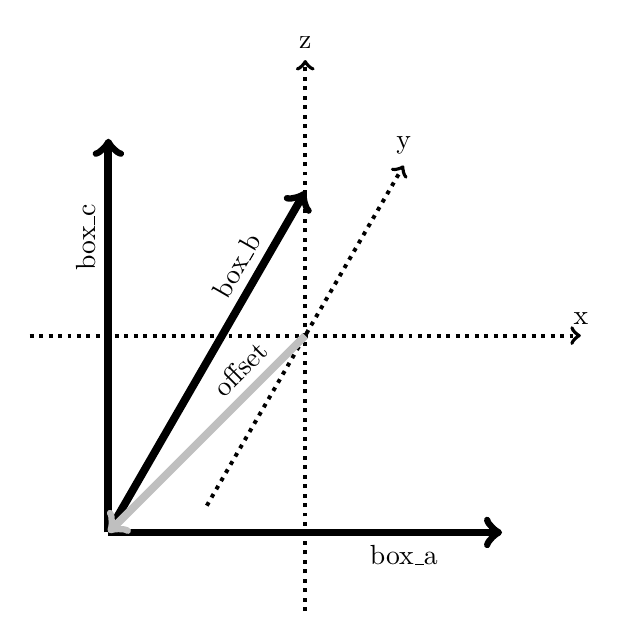
\begin{tikzpicture}
      \draw[->,black,line width=1mm] (-2.5,-2.5) -- (-2.5,2.5) node [near end,above,rotate=90] {box\_c};
      \draw[->,black,line width=1mm] (-2.5,-2.5) -- (0,1.83) node [near end,above,rotate=60] {box\_b};
      \draw[->,black,line width=1mm] (-2.5,-2.5) -- (2.5,-2.5) node [near end,below] {box\_a};

      \draw[->,black,dotted,line width=0.5mm] (-3.5,0) -- (3.5,0) node [left,above] {x};
      \draw[->,black,dotted,line width=0.5mm] (0,-3.5) -- (0,3.5) node [left,above] {z};
      \draw[->,black,dotted,line width=0.5mm] (-1.25,-2.16) -- (1.25,2.16) node [left,above] {y};

      \draw[->,lightgray,line width=1mm] (0,0) -- (-2.5,-2.5) node [near start,above,black,rotate=45] {offset};
\end{tikzpicture}
\end{center}
\caption{Scheme of system parameters describing the form and position of the simulation box}
\label{fig:interface_box_scheme}
\end{figure}

The common setup requires basic data about the simulation system. An overview can be seen in table \ref{tab:fcs_set_common_parameters}. The box vectors
describe the form of the box, in which the particles reside. For each solver there can be certain restrictions as for which kind of systems they can simulate. 
To get an idea which solvers work best (or work at all) with which systems please refer to the corresponding solver description within this documentation.
In general no solver is able to handle non-orthogonal boxes as of yet, although the interface should be able to handle these kind of boxes. The offset
enables the library to handle systems, which are shifted from the coordinate origin. For a graphical scheme, please refer to figure \ref{fig:interface_box_scheme}.
The use of periodicity is likewise restricted as the box forms. Not every solver is able to cope with every combination of periodicity. The only
common parameter not related to the system is the near field flag, which determines whether a method should perform its near field computations by itself or not.
By default, all solvers compute the interactions entirely by themselves. However, some solvers provide the possibility to delegate their near field 
computations to the main program. If the near field flag is set to false (i.e. 0), then interactions inside a solver-specific cutoff range are not computed.
The cutoff range can be retrieved (set) with a separate getter (setter) function. The solver methods provide separate potential functions for performing their
near field computations in the main program. The functionality of the near field flag is currently supported by methods P3M and P2NFFT.

\begin{table}
\begin{center}
\begin{tabular}{|p{0.2\textwidth}|p{0.45\textwidth}|p{0.25\textwidth}|}
          \hline
          parameter name        &       description                                         &   valid values                        \\
          \hline
          handle                &       pointer to parameter containing structure           &   FCS (C) or type (c\_ptr) (Fortran)   \\
          \hline
          near\_field\_flag    &       leave the near field calculations to the library    &   true ($\neq 0$) / false ($0$)       \\
          \hline
          box\_a                &       first vector describing the system box              &   $\in \mathbb{R}^3$                  \\
          \hline
          box\_b                &       second vector describing the system box             &   $\in \mathbb{R}^3$                  \\
          \hline
          box\_c                &       third vector describing the system box              &   $\in \mathbb{R}^3$                  \\
          \hline
          offset                &       offset of the lower front left corner from $\Vect{0}$&   $\in \mathbb{R}^3$                  \\
          \hline
          periodicity           &       periodicity of the system in each dimension (x,y,z) &   true / false                        \\
          \hline
          total\_particles      &       total amount of particles in the system             &   $\in \mathbb{N}^+$                  \\
          \hline 
\end{tabular}
\end{center}
\caption{Parameters for fcs\_common\_set}
\label{tab:fcs_set_common_parameters}
\end{table}

To change the solver-specific parameters, there are solver-specific setter functions. These are called \textit{fcs\_$<$solver$>$\_set\_$<$parameter$>$} where 
\textit{$<$solver$>$} is the abbreviation of the solver (table \ref{tab:solver_overview}) and parameter the name of the relevant parameter. If one wishes to change all parameters of
a solver, the use of \textit{fcs\_$<$solver$>$\_setup} is advised. A list of solver-specific parameters, that can be changed and possible values are available
in the chapters describing the solvers.

\subsection{Tuning Step}
\label{sec:tune_step}
\functiontoindex{fcs\_tune}



Most of the methods need a tuning step in which internal data structures are created according to the actual system that is simulated. Other methods
need information about the distribution of the particles within the system and between the processes. Therefore the tuning step is mandatory. In order
to tune the methods, the user has to call the function \textit{fcs\_tune} with the function call described in figure (\ref{fig:fcs_tune}). The function
calls awaits several input parameters and is similar to the function call of \textit{fcs\_run} described in the following section. First parameter of the
tuning is the handle, which was created in \textit{fcs\_init} (\ref{sec:init_step}) and then filled with \textit{fcs\_common\_set} (\ref{sec:par_setup}).
The parameter \textit{n\_locp} gives the number of particles on the local process, which is identical to the length of the array given as parameter 
\textit{charges}. For the array containing the charges, an array with thrice the length has to be supplied as parameter \textit{charges}. As final parameter,
the parameter \textit{n\_maxlocp} gives an estimation of the maximum number of particles being stored on the local process before the next call of the tuning
routine.\\
This routine is mandatory to be called, in order to grant a unified interface for the library. Some methods, e.g. PEPC, do not need this tuning step. But to be
able to switch the methods within a code without the need to greatly modify the code again, the tuning routine has to be called. If the user wants to use e.g. PEPC
as well as e.g. P2NFFT, he can use the same program (except for the method-specific setter routines), when including the tuning routine. 

\subsection{Calculation Step}
\label{sec:run_step}
\functiontoindex{fcs\_run}



The calculation step is the centerpiece of the library. Within it, the actual calculation of Coulomb interactions takes place. As mentioned in the description of tuning step,
the call to \textit{fcs\_run} (fig. \ref{fig:fcs_run}) is nearly the same, as for \textit{fcs\_tune} (see \ref{sec:tune_step}). There are two additional parameters, which are \textit{field} and
\textit{potential}. The first is the array to which the field data is added and has a size of thrice the number of local particles (\textit{n\_locp}), the latter
is the array in which the corresponding potentials are saved and has a size equal to the number of local particles (\textit{n\_locp}). All the other parameters
are equal to the parameters of \textit{fcs\_tune} (see above).


\subsection{Clean Up Step}
\label{sec:clean_up_step}
\functiontoindex{fcs\_destroy}



After the calculations are done, the memory allocated by the methods needs to be freed again. This task is done by the function \textit{fcs\_destroy} (fig. \ref{fig:fcs_destroy}).
As parameters only the FCS object is needed, in order to free memory allocated in connection with it, since the internal data structures of the methods are
administrated by those. The call to fcs\_destroy is not mandatory but the user is advised to call it, especially if he or she wants to repeat the calculation
with another method without restarting the program, since it cannot be guaranteed that more then one method can be used simultaneously without memory problems. 

\section{Error Handling}
\label{sec:error_handling}
\index{error handling}

Within the ScaFaCoS library a FCSResult type is defined. With this type return values and error messages of the methods and the interface routines are handled.
The type includes up to three pieces of information about error that have occurred during a call to a ScaFaCoS function. These pieces are a return code, an error
message and the source of the error within the library. As return values the values given in table \ref{tab:c_macros_error} can occur. In order to simplify the
error handling for the ScaFaCoS routines, the routines return \textit{NULL} as return value, instead of an allocated error object containing \textit{FCS\_SUCCESS}
as return value. The other information contained in the error type gives more information about the kind of error that occurred, e.g. if a method cannot handle
a certain system due to restrictions on periodicity, and where the error occurred within the library since the error can happen in functions called inside the
routine called by the user.\\
To get the information out of the error type, there are three functions for this task. Their calls are shown in figures \ref{fig:fcsResult_getReturnCode} to \ref{fig:fcsResult_getErrorSource}.
Due to restrictions in Fortran the message length in Fortran is capped to 256 characters.

\section{Fortran Specifics}

\begin{figure}[htb]
\begin{lstlisting}[language=Fortran,frame=trBL,breaklines,basicstyle=\small,prebreak={\raisebox{0ex}[0ex][0ex]{\ensuremath{\hookleftarrow}}}]
! Fortran
use iso_c_binding
character(kind = c_char, len = 32) :: string = "test_string"
string = trim(adjustl(string)) // c_null_char
\end{lstlisting}
\caption{Example for string truncation for strings used with ScaFaCoS}
\label{fig:example_string_fortran2c}
\end{figure}


In this section some advises are given for Fortran programmers. Since the Fortran interface is a wrapper interface above the C version of the interface trying to
stay as true to the C interface as possible, some things have to be observed. First it is advised to use the interoperable Fortran kinds delivered by the
library, which are \textit{fcs\_integer\_kind\_isoc} for integer and \textit{fcs\_real\_kind\_isoc}. With the usage of these kinds problems concerning the 
interoperability of the values is avoided. Secondly strings have to be terminated with C null characters and have to be trimmed to the correct length. An
example how this can be achieved is given in figure \ref{fig:example_string_fortran2c}. A third difference from Fortran to C is that in the Fortran interface
wherever possible the logical type is used instead of an integer value in C. This is true for every manual setter and getter connected to flags. In the parser
this exchange was not possible (see \ref{sec:interface_parser}).


\section{Further Functionality}

This sections describes some of the functionality the ScaFaCoS library has, which exceeds the pure calculation of Coulomb interactions. It also describes the
output functions within the library and the parser for parameters.

\label{sec:interface_functions}
\subsection{Near Field Solver}
\index{near field solver}
\label{sec:near_field_solver}

\todo[inline]{Should the near field solver be available to the user?}
Within the library a near field solver for given near field potentials is included. Some of the methods (P2NFFT and P3M) need to calculate separate near field
interactions, which is done by this solver. The solver uses a linked cell scheme for fast interaction calculation and uses the sorting library to create and
duplicate the particles (ghost-particles). It is able to handle periodicity and linked cell sizes that are smaller than the cut-off radius. With the near field
flag described in section \ref{sec:par_setup} the calculation of the near field portions of the Coulomb interactions can be delegated to external routines.
In order to do this the methods which support this (currently P3M and P2NFFT) provide a functions which can then be called from the user's program to calculate the
corresponding near field portions of the Coulomb interactions (see figure \ref{fig:fcs_compute_near_field} to \ref{fig:fcs_compute_near}). The aforementioned
functions are generic function that will calculate the according values for the chosen method. It is possible to check if the chosen method is able to relegate
the near field calculation by use of \textit{fcs\_method\_has\_near} (\ref{fig:fcs_method_has_near}).

\subsection{Optional Results}

It is possible to get additional results from the solver concerning the calculation. As of now the only additional result to have is the system virial. It is
possible that some solvers add additional optional results in the future. Since now only the virial is available here will be explained how to get the virial
from the solvers. For that two functions are needed, \textit{fcs\_require\_virial} (\ref{fig:fcs_require_virial}) and \textit{fcs\_get\_virial} (\ref{fig:fcs_get_virial}).
With \textit{fcs\_require\_virial} the user activates or deactivates the calculation of the virial. If set to true, the virial is activated, else it is not
calculated. If it is calculated, the user can get the calculated by the use of \textit{fcs\_get\_virial}. For that he has to pass an allocated array of nine
\textit{fcs\_float} values to the function.\\
Possibly in the next future other optional results will be implemented, if required by the community.

\subsection{Output of Interface Parameters}
\index{parameter output}
\functiontoindex{fcs\_printHandle}

For debugging purposes it is possible to print out the content of the FCS object. This is done by the use of the function \textit{fcs\_printContent} (figure \ref{fig:fcs_printHandle}).
The output shows the current values of the parameters set within the FCS object. If no changes were made to the solver-specific parameters, it shows the default
values for them. The behavior of the routine if used on a freshly created FCS object without set common parameters is undefined.

\subsection{Parser}
\index{parser}
\functiontoindex{fcs\_parser}
\label{sec:interface_parser}

To simplify the parameter input for programs basing on script file input, the ScaFaCoS library offers a parser that allows to read in parameters from a string.
The format of the passed string must adhere to the example shown in figure \ref{fig:parser_example}, while the function call can be seen in figure \ref{fig:fcs_parser}

\begin{figure}[htb]
\begin{lstlisting}[language=Fortran,frame=trBL,breaklines,basicstyle=\small,prebreak={\raisebox{0ex}[0ex][0ex]{\ensuremath{\hookleftarrow}}}]
string = "box_a,1.0,0.0,0.0,near_field_flag,1,pepc_theta,0.3"
\end{lstlisting}
\caption{Example of a parser string setting the first box vector, the near field flag and a method-specific parameter.}
\label{fig:parser_example}
\end{figure}

The format is an alteration of parameter name and value(s). In the example the first parameter to be set is a generic one, so no prefix is needed and the parameter
name is \textbf{box\_a}. Since the first box vector needs three floating point values, these are given after the parameter name, always separated by commas.
After the final parameter value, the next parameter name is expected, in the case of the example the parameter is another generic one, the \textbf{near\_field\_flag}.
Because this parameter needs only one integer value, it given and immediately followed by the next parameter name. The last parameter to be set is a solver-specific
one, the parameter \textbf{theta} from the PEPC solver. Since it is a PEPC-specific parameter, the solver name is added as a prefix, followed by the parameter name.
After it the parameter value follows, like with the generic parameters.\\
For Fortran users the advise, that every flag which is set with the parser, has to used the C syntax which requires an integer value (0 for false, 1 for true) instead
of \textit{.true.} or \textit{.false.}.

\FloatBarrier
\renewcommand\arraystretch{1.0}

\chapter{FMM -- Fast Multipole Method}
\label{cha:fmm}

\begin{verbatim}
Parameters

  - absrel: absolute or relative energy errors 
       0 = relative energy error 10^{-3} (default) 
       1 = absolute energy error deltaE 
       2 = relative energy error deltaE 

  - deltaE: relative or absolute energy error, depending on absrel
       absrel = 1: absolute total energy error 
       absrel = 2: relative energy error, 10^{-1}...10^{-14}

  - dipole_correction: type of dipole correction to use (explain!)
      currently ignored (not handed over by interface)
      -1 = no dipole correction
       0 = standard dipole correction
       1 = dipole correction activated
       default value?

Box Shape / Periodicity

  - open boundaries:               full support for any box shape

  - periodic or mixed boundaries:  support limited to cubic boxes;
                                   however, for mixed boundaries, 
                                   edges in non-periodic directions 
                                   may be shorter than periodic edges

Can Delegate Nearfield to MD:  no

Bugs / Missing Features

  - only backup version of virial tensor with periodic boundaries
  - can we lift the requirements for periodic or mixed boundaries
    to approximately cubic boxes, like for PEPC?
  - does not compile with Intel compiler
\end{verbatim}

\solvertoindex{Fast Multipole Method}
\solvertoindex{FMM}

%%% Local Variables: 
%%% mode: latex
%%% TeX-master: ug.tex
%%% End: 

 
\chapter{MEMD -- Maxwell Equation Molecular Dynamics}
\label{cha:memd}

\solvertoindex{MEMD}
\solvertoindex{Maxwell Equation Molecular Dynamics}

%%% Local Variables: 
%%% mode: latex
%%% TeX-master: ug.tex
%%% End: 


\chapter{MMM1D}
\label{cha:mmm1d}

\solvertoindex{MMM1D}

%%% Local Variables: 
%%% mode: latex
%%% TeX-master: ug.tex
%%% End: 


\chapter{MMM2D}
\label{cha:mmm2d}

\solvertoindex{MMM2D}

%%% Local Variables: 
%%% mode: latex
%%% TeX-master: ug.tex
%%% End: 


\chapter{Ewald}
\label{cha:ewald}

\solvertoindex{Ewald}

%%% Local Variables: 
%%% mode: latex
%%% TeX-master: ug.tex
%%% End: 

The well-known Ewald formula for the computation of \eqref{eq:ewald_potential} splits the
electrostatic potential $\phi$ into the following parts
\begin{equation}\label{eq:ewald}
 \phi = \phi^{\rm real} + \phi^{\rm reci}  + \phi^{\rm self}  + \phi^{\rm dipo},
\end{equation}
where the contribution from real space $ \phi^{\rm real}$, reciprocal space $\phi^{\rm reci}$,
the self-energy $\phi^{\rm self}$ and the dipole correction $\phi^{\rm dipo}$ are given by
\begin{eqnarray}
  \phi^{\rm real}(\mathbf x_j)
  &=& \nonumber
    \sum_{\mathbf r\in \mathbb Z^3}
    \underset{ l\neq j \,{\rm for}\, \mathbf r= \mathbf 0}{\sum_{l=1}^M}
    q_l\frac{{\rm erfc}(\alpha \|\mathbf x_j -\mathbf x_l +\mathbf r B\|_2)}{\|\mathbf x_j -\mathbf x_l +\mathbf r B\|_2},\\
  \phi^{\rm reci}(\mathbf x_j)
  &=& \label{eq:ewald_reci}
    \frac{1}{\pi B} \sum_{\mathbf k\in \mathbb Z^3\setminus\{\mathbf 0\}}
    \frac{{\rm e}^{-\pi^2 \|\mathbf k\|_2^2/(\alpha B)^2}}{\|\mathbf k\|_2^2}
    \sum_{l=1}^M q_l {\rm e}^{-2\pi {\rm i} \mathbf k (\mathbf x_j -\mathbf x_l)/B}\, ,\\
  \phi^{\rm self} (\mathbf x_j)
  &=&
    -2 q_j \frac{\alpha}{\sqrt{\pi}}\; ,\nonumber  \\
  \widetilde\phi^{\rm dipo}
  &=&
    \frac{2\pi}{3V}\bigg(\sum_{l=1}^Mq_{l}\mathbf x_{l}\bigg)^{2}\; .\nonumber %\label{eq:E_dipol_part}
\end{eqnarray}
Thereby, the complementary error function is defined by $\textrm{erfc}(z) =
\frac{2}{\sqrt{\pi}}\int_z^\infty {\rm e}^{-t^2} {\rm d}t$.
Choosing optimal parameters, Ewald summation scales as ${\cal O}(M^{3/2})$ \cite{kolafa92a}.
\chapter{P2NFFT -- Particle-Particle NFFT}
\label{cha:p2nfft}

\solvertoindex{P2NFFT}
\solvertoindex{Particle-Particle NFFT}

\def\alp{13}


%%% Local Variables: 
%%% mode: latex
%%% TeX-master: ug.tex
%%% End: 


P2NFFT is a common framework for almost all FFT based fast Coulomb solvers.
The computation of Coulomb interactions is split into a short range interaction (near field) and
a long range interaction (far field).
For sake of simplicity, we describe the idea of P2NFFT only for the one-dimensional case.
In addition, we do not stress all the details, that arise from the difference between periodic and
non-periodic boundary conditions. More detailed descriptions of the algorithms can be found in \cite{PiPo10}.

\section{Description of the Method}

As usual, we assume $M$ charges $q_l$ at position $r_l$. The potentials $\phi_j$ at position $r_j$
are given by
\begin{equation*}
  \phi_j
  =
  \sideset{}{^\prime}\sum_{l=1}^M
    q_l\frac{1}{r_{jl}}
  \,,
\end{equation*}
and the Electrostatic fields $E_j$ at position $r_j$ are given by
\begin{equation*}
  E_j
  =
  \sideset{}{^\prime}\sum_{l=1}^M
    q_l\nabla\frac{1}{r_{jl}}
  =
  \sideset{}{^\prime}\sum_{l=1}^M
    q_l \frac{r_l}{r_{jl}}
  \,.
\end{equation*}
Hereby, the distance between two particles at positions $r_j$ and $r_l$ is given by $r_{jl}:=|r_j-r_l|$.

\subsection{Periodic boundary conditions}
In this section we present a straightforward method, that accelerates the traditional Ewald
summation technique by NFFT. This combination was first presented in \cite{HeLa06} and
is very similar to the FFT-accelerated Ewald sums, namely, the so-called
particle-particle particle-mesh (P$^3$M), particle-mesh Ewald (PME) and smooth particle-mesh
Ewald (SPME), see also \cite{DeHo98a}.
Additionally we will see, that the accelerated Ewald summation can be reinterpreted
into a method very similar to our fastsum Algorithm~\ref{algo:fastsum}.


In order to overcome this increase in time we apply the NFFT for the calculation of the
reciprocal-space potential  $\phi^{\rm reci}$ and we obtain a method similar as our fast summation method.
To this end, we compute the Fourier transformed charge density
\begin{equation*}
 S(\mathbf k) = \sum_{l=1}^M q_l {\rm e}^{+2\pi {\rm i} \mathbf k \mathbf x_l/B}
\end{equation*}
by NFFT$^\adj$ and after truncation of the sum \eqref{eq:ewald_reci} we obtain by NFFT
\begin{equation*}
 \phi^{\rm reci}(\mathbf x_j) \approx
 \frac{1}{\pi B} \sum_{\mathbf k\in I_{\mathbf N}\setminus\{\mathbf 0\}}
 \frac{{\rm e}^{-\pi^2 \|\mathbf k\|_2^2/(\alpha B)^2}}{\|\mathbf k\|_2^2}
 S(\mathbf k){\rm e}^{-2\pi {\rm i} \mathbf k \mathbf x_j/B}\, .
\end{equation*}





\subsection{Calculation of the Potentials}

\begin{figure}[htb]
  \centering
  \beginmypgfhack{p2nfft_ewald_split}
%   \beginpgfgraphicnamed{p2nfft_ewald_split}
  \begin{tikzpicture}
    \node (plot_one_over_r) [right]{
      \begin{tikzpicture}
        \begin{axis}[tiny, xmin=0, xmax=0.5, ymin=0, ymax=17]
          \addplot gnuplot [id=erf,mark=none,domain=0:0.5, samples = 101, very thick, black]{(x==0) ? 100 : 1/x};
        \end{axis}
      \end{tikzpicture}
    };
    \node (plot_equals) at (plot_one_over_r.east) [right]{=};
    \node (plot_erfc) at (plot_equals.east) [right]{
      \begin{tikzpicture}
        \begin{axis}[tiny, xmin=0, xmax=0.5, ymin=0, ymax=17]
          \addplot gnuplot [id=erf,mark=none,domain=0:0.5, samples = 101, very thick, black]{(x==0) ? 100 : 1/x};
          \addplot gnuplot [id=erf,mark=none,domain=0:0.5, samples = 101, very thick, blue]{(x==0) ? 100 : erfc(x*\alp)/x};
        \end{axis}
%         \node [xshift=8ex, yshift=9ex] {\tiny$\alpha=\alp$};
      \end{tikzpicture}
    };
    \node (plot_plus) at (plot_erfc.east) [right]{+};
    \node (plot_erf) at (plot_plus.east) [right]{
      \begin{tikzpicture}
        \begin{axis}[tiny, xmin=0, xmax=0.5, ymin=0, ymax=17]
          \addplot gnuplot [id=erf,mark=none,domain=0:0.5, samples = 101, very thick, black]{(x==0) ? 100 : 1/x};
          \addplot gnuplot [id=erf,mark=none,domain=0:0.5, samples = 101, very thick, red]{(x==0) ? 2*\alp/sqrt(pi) : erf(x*\alp)/x};
        \end{axis}
%         \node [xshift=8ex, yshift=9ex] {\tiny$\alpha=\alp$};
      \end{tikzpicture}
    };
    \node (eqn_one_over_r) at (plot_one_over_r.north) [above]{
      $\tfrac{1}{r}$
    };
    \node (eqn_erfc) at (plot_erfc.north) [above]{
      \color{blue}$\tfrac{1}{r} - R(r)$
    };
    \node (eqn_erf) at (plot_erf.north) [above]{
      \color{red}$R(r)$
    };
    \node (eqn_equals) at (plot_equals.north) [above=7ex]{=};
    \node (eqn_plus) at (plot_plus.north) [above=7ex]{+};
  \end{tikzpicture}
  \endmypgfhack
%   \endpgfgraphicnamed
  \caption{Splitting of Coulomb potential into near field (blue) and far field (red).}
\end{figure}

\begin{equation*}
  \phi(r_j)
  =
  \sideset{}{^\prime}\sum_{l=1}^M
    \frac{q_l}{r_{jl}}
  =
  R(0) + \sideset{}{^\prime}\sum_{l=1}^M
    q_l \left( \frac{1}{r_{jl}} - R(r_{jl}) \right)
  - \sum_{l=1}^M
    q_l R(r_{jl})
  \,,\quad j=1,\hdots,M
\end{equation*}



\begin{equation*}
  R(r)
  \approx
    \sum_{k=-N/2}^{N/2-1} \hat R_k \eim{kr}
\end{equation*}

\begin{equation*}
  \sum_{l=1}^M
    q_l R(r_{jl})
  \approx
  \sum_{l=1}^M q_l
    \sum_{k=-N/2}^{N/2-1} \hat R_k \eim{kr_{jl}}
  =
  \sum_{k=-N/2}^{N/2-1} \hat R_k
    \left(
      \sum_{l=1}^M q_l \eip{kr_l}
    \right)
    \eim{kr_j}
\end{equation*}

Near field interactions are computed with the ScaFaCoS near field solver, but can also be redirected to any other the near field solver.

Far field interactions are computed via convolution in Fourier space.
With the appropriate choice of window functions and convolutions in Fourier space,
P2NFFT becomes the P3M (default for fully periodic boundaries), the NFFT based fast summation (default for fully non-periodic boundaries)
or almost any other FFT based fast Coulomb solver like PME, SPME, Gaussian split Ewald or plain Ewald summation.
Note, that an uniform particle distribution is required in order to achieve the typical $\mathcal{O}(N\log N)$ scaling.

\subsection{Calculation of the Electrostatic Fields}

\subsection{Calculation of the Virial}






\newpage
\section{Features}

\begin{description}
\item[Periodicity:] Only fully periodic and fully non-periodic boundaries are supported.
\item[Box shape:] Only cubic box shape is supported.
\item[Autotuning:] For fully periodic boundaries, the parameters can be automatically tuned when a
  required tolerance in the absolute rms field error is provided. For fully non-periodic boundaries,
  the parameters are more or less intelligently guessed when a required tolerance in the absolute
  potential error is provided.  
\item[Delegate near-field:] Yes.
\item[Virial:] Yes for fully non-periodic boundaries. For fully periodic boundaries we only compute an approximation of
  the diagonal of the virial tensor, \ie, all entries of the diagonal are set equal to one third of the total energy.
\end{description}

\section{Solver-specific Parameters}
The tolerance parameters are common to all ScaFaCoS solvers. At the moment P2NFFT only supports automatic parameter tuning for the following tolerance types.
\begin{itemize}
  \item \verb!tolerance_type! -
    The type of error that we want to check for. Allowed values are \verb!FCS_TOLERANCE_TYPE_FIELD! (absolute rms error in the fields)
    for fully periodic boundaries and \verb!FCS_TOLERANCE_TYPE_POTENTIAL! (absolute rms error in the potentials) for non-periodic boundaries.
  \item \verb!tolerance! -
    The allowed tolerance of the error. Type of the error is given by \verb!tolerance_type!. If the required tolerance can't be achieved
    with the given parameters, P2NFFT aborts with an error message.
\end{itemize}

In addition, P2NFFT offers the following parameters, which can be adjusted by the P2NFFT-specific functions described in the next section.
Alternatively, you can use the ScaFaCoS test program together with the optional command line argument \verb!-c! and a comma separated list
of parameter settings, e.g., use
\begin{verbatim}
./scafacos_test p2nfft systems/3d-periodic/cloud_wall.xml.gz \
-c tolerance_field,1e-4,p2nfft_r_cut,4.5,pnfft_N,16,16,16,pfft_patience,0
\end{verbatim}
in order to run the test program with a near field cut off range of $4.5$ and a sloppy planned FFT of size $16\times 16 \times 16$ up to tolerance $10^{-4}$ in the fields.
\begin{itemize}
  \item \verb!p2nfft_r_cut! -
    Absolute cutoff distance of the near field. Can be
    automatically tuned. Feasible values are in the order of the mean
    free path between the two nearest charges.
    \verb!p2nfft_r_cut! has to be less than half the
    smallest simulation box length.  When \verb!p2nfft_r_cut! is chosen too
    small, the errors of the algorithm become large, the required
    accuracy might not be achieved, or the grid has to be chosen very
    large, which will slow down the algorithm.  When \verb!p2nfft_r_cut! is
    chosen too large, the algorithm might become slow as most
    computation is done in the near field region.
    This parameter corresponds to \verb!r_cut! of the P3M solver.
  \item \verb!p2nfft_epsI! -
    Relative cutoff distance of the near field. P2NFFT scales the original box size into a cube of side length 1.
    For fully periodic boundary conditions this corresponds to a simple scaling by the box size. However, the scaling is more complicated if non-periodic
    boundary conditions are involved. Application of the same scaling factor on \verb!r_cut! gives \verb!epsI!.
  \item \verb!p2nfft_alpha! -
    Ewald splitting parameter. Can be automatically tuned.
    This parameter corresponds to \verb!alpha! of the P3M solver.
  \item \verb!p2nfft_cao! -
    Charge assignment order. Can be automatically tuned. This parameter mostly corresponds to \verb!cao! of the P3M solver.
    However, note that this is only a wrapper that sets \verb!pnfft_m! to the value \verb!(p2nfft_cao+1)/2! (division rounded down).
    Therefore, P2NFFT will always use an even charge assignment order.
  \item \verb!p2nfft_intpol_order! -
    P2NFFT uses interpolation tables to speed up the repeated computation of the near field correction. The order of interpolation is given by \verb!intpol_order!.
    Feasible values are $-2$ (approximation of the error function according to \cite[eq.~(7.1.26)]{AbSt72}, which yields an error of $1.5\times 10^{-7}$),
    $-1$ (direct evaluation of the error function), $0$ (constant interpolation), $1$ (linear interpolation), $2$ (quadratic interpolation) and $3$ (cubic interpolation).
    Default value is $3$.
  \item \verb!p2nfft_reg! -
    Choose between the two regularization methods for non-periodic boundaries. Feasible values are \verb!2ptaylor! (Regularization with 2-point-Taylor polynomials)
    and \verb!cg! (Fourier coefficients have been precomputed via CG iteration). Default is \verb!cg!
  \item \verb!p2nfft_p! -
    The degree of the two-point-Taylor polynomial. This parameter only takes affect, if regularization \verb!2ptaylor! has been enabled.
    Feasible values are any integers between $1$ and $16$. Default value is $7$.
  \item \verb!p2nfft_virial! -
    Decide if the computation of the virial should be included in P2NFFT.
    Feasible values are $0$ (disable virial computation), or any other integer (enable virial computation).
    Default value is $0$ (disable virial computation).
  \item \verb!p2nfft_ignore_tolerance! -
    On default, P2NFFT aborts with an error message, if the required error tolerance can not be reached.
    This flag disables the check for accuracy and gives the possibility to run P2NFFT
    with any set of parameters. It is intended for very experienced users that tune all parameters manually.
    Default value is $0$ (abort if tolerance check fails). Any other value disables the tolerance check.
\end{itemize}

\subsection{PNFFT-specific Parameters}
\begin{itemize}
  \item \verb!pnfft_N! (acronym: \verb!p2nfft_grid!) -
    Size of the FFT grid. Can be automatically tuned.
    Feasible values are in the order of $M^{1/3}$, \ie, one
    grid point for each particle. The grid size may be any positive integer, but powers of
    two are recommended. The larger the grid, the smaller the
    error, but also the higher the memory and computational requirements
    of the algorithm.
    This parameter corresponds to the FFT grid size (\verb!grid!) of the P3M solver.
  \item \verb!pnfft_n! (acronym: \verb!p2nfft_oversampled_grid!) -
    Size of the oversampled FFT grid. Can be automatically tuned.
    Especially for non-periodic boundaries it is necessary to introduce oversampling to reduce the aliasing error.
    Feasible values are any integer $\verb!n! \ge \verb!N!$. Default value is
    \verb!N! for fully periodic boundaries and 2\verb!N! for fully non-periodic
    boundaries.
  \item \verb!pnfft_window! (alternative: \verb!pnfft_window_name!) -
    NFFT window function. Feasible values are $0$ (Kaiser-Bessel window), $1$ (Gaussian window),
    $2$ (B-spline window), $3$ (Sine Cardinal window - Fourier transform of the B-spline window) and $4$
    (window function based on the modified Bessel function of first kind - Fourier transform of the Kaiser-Bessel window).
    Default value is $2$ (B-spline). Recommended values are $0$ (Kaiser-Bessel) for fully non-periodic boundaries and $2$ (B-spline) for fully periodic boundaries.
  \item \verb!pnfft_window_name! (alternative: \verb!pnfft_window!) -
    Name of the NFFT window function. Feasible values are \verb!kaiser! (Kaiser-Bessel window), \verb!gaussian! (Gaussian window),
    \verb!bspline! (B-spline window), \verb!sinc! (Sine Cardinal window - Fourier transform of the B-spline window) and \verb!bessel_i0!
    (window function based on the modified Bessel function of first kind - Fourier transform of the Kaiser-Bessel window).
    Default value is \verb!bspline!. Recommended values are \verb!kaiser! for fully non-periodic boundaries and \verb!bspline! for fully periodic boundaries.
  \item \verb!pnfft_m! (see also: \verb!p2nfft_cao!) -
    Real space cutoff of the window function. The number of grid points that are influenced
    by a charged particle. Can be automatically tuned. Allowed values are any positive integers.
    In most cases \verb!m! is chosen between $1$ (low precision) and $16$ (very high precision).\\
    {\bfseries Note: Due to historical reasons, this parameter corresponds to one half of the charge assignment order
    (\verb!cao!) of the P3M solver!}
  \item \verb!pnfft_intpol_order! -
    PNFFT uses interpolation tables to speed up the repeated evaluation of the window functions. The integer \verb!pnfft_intpol_order! gives the interpolation order.
    Feasible values are $-1$ (direct evaluation of window function without interpolation), $0$, (constant interpolation), $1$ (linear interpolation), $2$ (quadratic interpolation) and $3$ (cubic interpolation).
    Default value is $3$ (cubic interpolation).
  \item \verb!pnfft_pre_phi_hat! -
    Flag to enable precomputed Fourier coefficients for faster computation of the diagonal matrix in the NFFT algorithm.
    Feasible values are $0$ (turn off pre-computation), or any other integer \verb!pnfft_pre_phi_hat!$\ne0$ (enable pre-computation).
    Default value is $1$ (enable pre-computation).
  \item \verb!pnfft_fg_psi! -
    Set PNFFT flag \verb!PNFFT_FG_PSI!. Only Gaussian window function we can use Fast Gaussian Gridding in order to speed up the evaluation of the window function.
    Feasible values are $0$ (switch Fast Gaussian gridding off), or any other integer \verb!pnfft_fg_psi!$\ne0$ (use Gaussian gridding).
    Default value is $0$ (since B-Spline is the default window function).
  \item \verb!pnfft_fft_in_place! -
    Set PNFFT flag \verb!PNFFT_FFT_IN_PLACE!. This causes the PNFFT planner to use in-place-FFTs, which saves about half of the memory for FFT but may sacrifices some performance.
    Feasible values are $0$ (call out-of-place FFTs), or any other integer \verb!pnfft_fft_in_place!$\ne0$ (call in-place-FFTs).
    Default value is \verb!pnfft_fft_in_place!$=0$ (call out-of-place FFTs).
  \item \verb!pnfft_sort_nodes! -
    Set PNFFT flag \verb!PNFFT_SORT_NODES!. Chooses whether to call a local sort before the interpolation step. This may result in better cache locality.
    Feasible values are $0$ (omit local sort), or any other integer \verb!pnfft_sort_nodes!$\ne0$ (sort before interpolation).
    Default value is \verb!pnfft_sort_nodes!$=0$ (omit local sort).
  \item \verb!pnfft_interlaced! -
    Set PNFFT flag \verb!PNFFT_INTERLACED!. Chooses whether PNFFT uses interlacing. This gives better accuracy at the price of more operations.
    Feasible values are $0$ (omit interlacing), or any other integer \verb!pnfft_interlaced!$\ne0$ (enable interlacing).
    Default value is \verb!pnfft_interlaced!$=0$ (omit interlacing).
  \item \verb!pnfft_grad_ik! -
    Set PNFFT flag \verb!PNFFT_GRAD_IK!. Chooses whether PNFFT computes the gradient through multiplication with $-2\pi\textrm{i}\mathbf{k}$ in Fourier space.
    This gives better accuracy in comparison to analytic differentiation at the price of more operations. Especially, we have to call four backward FFTs (instead of one for analytic differentiation).
    Feasible values are $0$ (use analytic differentiation), or any other integer \verb!pnfft_grad_ik!$\ne0$ (use Fourier space differentiation).
    Default value is \verb!pnfft_grad_ik!$=0$ (use analytic differentiation).
  \item \verb!pnfft_pre_psi! -
    Set PNFFT flag \verb!PNFFT_PRE_PSI!. Tensor product based precomputation of the window function. This option reduces the amount of repeated evaluations of the window function at the cost of
    $6(2m+1)M$ floats (or $3(2m+1)M$ floats if the gradient is not needed).
    Since the this kind of precomputation depends on the nodes $\mathbf x_j$, it must be performed during \verb!fcs_run! instead of \verb!fcs_tune!.
    Feasible values are $0$ (switch off precomputation), or any other integer \verb!pnfft_pre_psi!$\ne0$ (switch on precomputation).
    Default value is $0$ (no precomputation). This flag can not be used together with \verb!pnfft_pre_full_psi!.
  \item \verb!pnfft_pre_fg_psi! -
    Set PNFFT flags \verb!PNFFT_FG_PSI! and \verb!PNFFT_PRE_PSI!, i.e., use Fast Gaussian Gridding for tensor product based precomputation.
    Since the this kind of precomputation depends on the nodes $\mathbf x_j$, it must be performed during \verb!fcs_run! instead of \verb!fcs_tune!.
    Feasible values are $0$ (switch off precomputation), or any other integer \verb!pnfft_pre_fg_psi!$\ne0$ (switch on precomputation).
    Default value is $0$ (no precomputation). This flag can not be used together with \verb!pnfft_pre_full_psi!.
  \item \verb!pnfft_pre_full_psi! -
    Set PNFFT flag \verb!PNFFT_PRE_FULL_PSI!. Full precomputation of the window function. This option reduces the amount of repeated evaluations of the window function at the cost of
    $4(2m+1)^3M$ floats (or $(2m+1)^3M$ floats if the gradient is not needed).
    Since the this kind of precomputation depends on the nodes $\mathbf x_j$, it must be performed during \verb!fcs_run! instead of \verb!fcs_tune!.
    Feasible values are $0$ (switch off precomputation), or any other integer \verb!pnfft_pre_psi!$\ne0$ (switch on precomputation).
    Default value is $0$ (no precomputation). This flag can not be used together with \verb!pnfft_pre_full_psi!.
  \item \verb!pnfft_pre_full_fg_psi! -
    Set PNFFT flags \verb!PNFFT_FULL_FG_PSI! and \verb!PNFFT_PRE_FULL_PSI!, i.e., use Fast Gaussian Gridding for full window function precomputation.
    Since the this kind of precomputation depends on the nodes $\mathbf x_j$, it must be performed during \verb!fcs_run! instead of \verb!fcs_tune!.
    Feasible values are $0$ (switch off precomputation), or any other integer \verb!pnfft_pre_full_fg_psi!$\ne0$ (switch on precomputation).
    Default value is $0$ (no precomputation). This flag can not be used together with \verb!pnfft_pre_psi!.
  \item \verb!pnfft_real_f! -
    Set PNFFT flag \verb!PNFFT_REAL_F!. Normally, PNFFT works on complex valued inputs. This flag enables some optimizations for real valued inputs, e.g., substituting complex additions and multiplications with real ones.
    However, this comes at the price of strided memory access and does not always improve performance.
    Feasible values are $0$ (use complex operations), or any other integer \verb!pnfft_real_f!$\ne0$ (use real operations where possible).
    Default value is \verb!pnfft_real_f!$=0$ (use complex operations).
\end{itemize}

\subsection{PFFT-specific Parameters}
\begin{itemize}
  \item \verb!pfft_patience! -
    Similar to FFTW, the PFFT library splits the computation of parallel FFT into a more or less time consuming planning step and a fast execution step.
    The time spent for planning can be adjusted by the \verb!pfft_patience! flag. Feasible values are $0$ (plan PFFT with \verb!PFFT_ESTIMATE!), $1$ (plan PFFT with \verb!PFFT_MEASURE!),
    $2$ (plan PFFT with \verb!PFFT_PATIENT!) and $3$ (plan PFFT with \verb!PFFT_EXHAUSTIVE!). All other values raise an error. Default value is $1$ (\verb!PFFT_MEASURE!).
  \item \verb!pfft_tune! -
    The PFFT library uses FFTW for computing serial FFTs combined with serial transpositions. Sometimes its better to perform the FFT and transposition in two separate steps,
    but the FFTW planner does not recognize. For value \verb!pfft_tune!$=0$ PFFT uses the FFTW plan as it is. For any other value, PFFT calls an additional planner in order to decide
    if performance gets better when the local FFT and transposition is performed in two separate steps. For large local array sizes this tuning gets very time consuming.
    Default value is $0$ (tuning turned off).
  \item \verb!pfft_preserve_input! -
    PFFT can chose between a larger set of algorithms, if it is allowed to overwrite the input array.
    Feasible values are $0$ (PFFT is allowed to destroy input), or any other integer \verb!pfft_preserve_input!$\ne0$ (PFFT is not allowed to destroy input).
    Default value is $0$ (PFFT is allowed to destroy input).
\end{itemize}


\section{Solver-specific Functions}
\begin{itemize}
  \item
\begin{alltt}
FCSResult fcs_p2nfft_set_r_cut(FCS handle, fcs_float r_cut);
FCSResult fcs_p2nfft_get_r_cut(FCS handle, fcs_float* r_cut);
FCSResult fcs_p2nfft_set_r_cut_tune(FCS handle);
\end{alltt}
    Set/restore/retrieve absolute near field cutoff radius.
  \item
\begin{alltt}
FCSResult fcs_p2nfft_set_epsI(FCS handle, fcs_float eps_I);
FCSResult fcs_p2nfft_get_epsI(FCS handle, fcs_float* eps_I);
FCSResult fcs_p2nfft_set_epsI_tune(FCS handle);
\end{alltt}
    Set/restore/retrieve relative near field cutoff radius.
  \item
\begin{alltt}
FCSResult fcs_p2nfft_set_alpha(FCS handle, fcs_float alpha);
FCSResult fcs_p2nfft_get_alpha(FCS handle, fcs_float* alpha);
FCSResult fcs_p2nfft_set_alpha_tune(FCS handle);
\end{alltt}
    Set/restore/retrieve Ewald splitting parameter.
  \item
\begin{alltt}
FCSResult fcs_p2nfft_set_interpolation_order(
    FCS handle, fcs_int intpol_order);
FCSResult fcs_p2nfft_get_interpolation_order(
    FCS handle, fcs_int* intpol_order);
\end{alltt}
    Set/retrieve interpolation order of near field correction (optional, default = 3).
  \item
\begin{alltt}
FCSResult fcs_p2nfft_set_regularization(FCS handle, fcs_int reg);
FCSResult fcs_p2nfft_get_regularization(FCS handle, fcs_int* reg);
FCSResult fcs_p2nfft_set_regularization_by_name(
    FCS handle, char* reg_name);
\end{alltt}
    Set/retrieve the near field regularization by number or name (default = 0).
    Feasible values are 0 (\verb!"cg"!) and 1 (\verb!"2ptaylor"!).
  \item
\begin{alltt}
FCSResult fcs_p2nfft_set_p(FCS handle, fcs_int p);
FCSResult fcs_p2nfft_get_p(FCS handle, fcs_int* p);
FCSResult fcs_p2nfft_set_p_tune(FCS handle);
\end{alltt}
    Set/restore/retrieve polynomial degree of two-point-Taylor regularization.
  \item
\begin{alltt}
FCSResult fcs_p2nfft_require_virial(
    FCS handle, fcs_int require_virial);
\end{alltt}
    Enable virial computation (optional, default = 0).
\begin{alltt}
FCSResult fcs_p2nfft_get_virial(FCS handle, fcs_float* virial);
\end{alltt}
    Retrieve virial (optional, default)
\begin{alltt}
FCSResult fcs_p2nfft_virial_is_active(
    FCS handle, fcs_int* yes_or_no);
\end{alltt}
    Check if virial computation is enabled.
  \item
\begin{alltt}
FCSResult fcs_p2nfft_set_ignore_tolerance(
    FCS handle, fcs_int set_ignore_tolerance);
FCSResult fcs_p2nfft_get_ignore_tolerance(
    FCS handle, fcs_int* set_ignore_tolerance);
\end{alltt}
    Set/retrieve flag for disabling the accuracy check (default = 0).
  \item
\begin{alltt}
FCSResult fcs_p2nfft_set_grid(
    FCS handle, fcs_int N0, fcs_int N1, fcs_int N2);
FCSResult fcs_p2nfft_get_grid(
    FCS handle, fcs_int* N0, fcs_int* N1, fcs_int* N2);
FCSResult fcs_p2nfft_set_grid_tune(FCS handle);
\end{alltt}
    Set/restore/retrieve FFT grid size.
  \item
\begin{alltt}
FCSResult fcs_p2nfft_set_oversampled_grid(
    FCS handle, fcs_int n0, fcs_int n1, fcs_int n2);
FCSResult fcs_p2nfft_get_oversampled_grid(
    FCS handle, fcs_int* n0, fcs_int* n1, fcs_int* n2);
FCSResult fcs_p2nfft_set_oversampled_grid_tune(FCS handle);
\end{alltt}
    Set/restore/retrieve oversampled FFT grid size.
  \item
\begin{alltt}
FCSResult fcs_p2nfft_set_cao(FCS handle, fcs_int cao);
FCSResult fcs_p2nfft_get_cao(FCS handle, fcs_int* cao);
FCSResult fcs_p2nfft_set_cao_tune(FCS handle);
\end{alltt}
    Set/restore/retrieve real space cutoff of window function.
\end{itemize}

\subsection{PNFFT-specific Functions}
\begin{itemize}
  \item
\begin{alltt}
FCSResult fcs_p2nfft_set_pnfft_N(
    FCS handle, fcs_int N0, fcs_int N1, fcs_int N2);
FCSResult fcs_p2nfft_get_pnfft_N(
    FCS handle, fcs_int* N0, fcs_int* N1, fcs_int* N2);
FCSResult fcs_p2nfft_set_pnfft_N_tune(FCS handle);
\end{alltt}
    Set/restore/retrieve FFT grid size.
  \item
\begin{alltt}
FCSResult fcs_p2nfft_set_pnfft_n(
    FCS handle, fcs_int n0, fcs_int n1, fcs_int n2);
FCSResult fcs_p2nfft_get_pnfft_n(
    FCS handle, fcs_int* n0, fcs_int* n1, fcs_int* n2);
FCSResult fcs_p2nfft_set_pnfft_n_tune(FCS handle);
\end{alltt}
    Set/restore/retrieve oversampled FFT grid size.
  \item
\begin{alltt}
FCSResult fcs_p2nfft_set_pnfft_window(
    FCS handle, fcs_int window);
FCSResult fcs_p2nfft_get_pnfft_window(
    FCS handle, fcs_int* window);
FCSResult fcs_p2nfft_set_pnfft_window_by_name(
    FCS handle, char* window_name );
\end{alltt}
    Set/retrieve \verb!pnfft_window! by number or name. (optional, default = 1).
    Feasible values are 0 (\verb!"gaussian"!), 1 (\verb!"bspline"!), 2 (\verb!"sinc"!), 3 (\verb!"kaiser"!) and 4 (\verb!"bessel_i0"!).
  \item
\begin{alltt}
FCSResult fcs_p2nfft_set_pnfft_m(FCS handle, fcs_int m);
FCSResult fcs_p2nfft_get_pnfft_m(FCS handle, fcs_int* m);
FCSResult fcs_p2nfft_set_pnfft_m_tune(FCS handle);
\end{alltt}
    Set/restore/retrieve real space cutoff of window function.
  \item
\begin{alltt}
FCSResult fcs_p2nfft_set_pnfft_interpolation_order(
    FCS handle, fcs_int intpol_order);
FCSResult fcs_p2nfft_get_pnfft_interpolation_order(
    FCS handle, fcs_int* intpol_order);
\end{alltt}
    Set/retrieve \verb!pnfft_intpol_order! (optional, default = 3).
  \item
\begin{alltt}
FCSResult fcs_p2nfft_set_pnfft_pre_phi_hat(
    FCS handle, fcs_int yes_or_no);
FCSResult fcs_p2nfft_get_pnfft_pre_phi_hat(
    FCS handle, fcs_int* yes_or_no);
\end{alltt}
    Set/retrieve flag \verb!pnfft_pre_phi_hat! (optional, default = 0).
  \item
\begin{alltt}
FCSResult fcs_p2nfft_set_pnfft_fg_psi(
    FCS handle, fcs_int yes_or_no);
FCSResult fcs_p2nfft_get_pnfft_fg_psi(
    FCS handle, fcs_int* yes_or_no);
\end{alltt}
    Set/retrieve flag \verb!pnfft_fg_psi! (optional, default = 0).
  \item
\begin{alltt}
FCSResult fcs_p2nfft_set_pnfft_fft_in_place(
    FCS handle, fcs_int yes_or_no);
FCSResult fcs_p2nfft_get_pnfft_fft_in_place(
    FCS handle, fcs_int* yes_or_no);
\end{alltt}
    Set/retrieve flag \verb!pnfft_fft_in_place! (optional, default = 0).
  \item
\begin{alltt}
FCSResult fcs_p2nfft_set_pnfft_sort_nodes(
    FCS handle, fcs_int yes_or_no);
FCSResult fcs_p2nfft_get_pnfft_sort_nodes(
    FCS handle, fcs_int* yes_or_no);
\end{alltt}
    Set/retrieve flag \verb!pnfft_sort_nodes! (optional, default = 0).
  \item
\begin{alltt}
FCSResult fcs_p2nfft_set_pnfft_interlaced(
    FCS handle, fcs_int yes_or_no);
FCSResult fcs_p2nfft_get_pnfft_interlaced(
    FCS handle, fcs_int* yes_or_no);
\end{alltt}
    Set/retrieve flag \verb!pnfft_interlaced! (optional, default = 0).
  \item
\begin{alltt}
FCSResult fcs_p2nfft_set_pnfft_grad_ik(
    FCS handle, fcs_int yes_or_no);
FCSResult fcs_p2nfft_get_pnfft_grad_ik(
    FCS handle, fcs_int* yes_or_no);
\end{alltt}
    Set/retrieve flag \verb!pnfft_grad_ik! (optional, default = 0).
  \item
\begin{alltt}
FCSResult fcs_p2nfft_set_pnfft_pre_psi(
    FCS handle, fcs_int yes_or_no);
FCSResult fcs_p2nfft_get_pnfft_pre_psi(
    FCS handle, fcs_int* yes_or_no);
\end{alltt}
    Set/retrieve flag \verb!pnfft_pre_psi! (optional, default = 0).
  \item
\begin{alltt}
FCSResult fcs_p2nfft_set_pnfft_pre_fg_psi(
    FCS handle, fcs_int yes_or_no);
FCSResult fcs_p2nfft_get_pnfft_pre_fg_psi(
    FCS handle, fcs_int* yes_or_no);
\end{alltt}
    Set/retrieve flag \verb!pnfft_pre_fg_psi! (optional, default = 0).
  \item
\begin{alltt}
FCSResult fcs_p2nfft_set_pnfft_pre_full_psi(
    FCS handle, fcs_int yes_or_no);
FCSResult fcs_p2nfft_get_pnfft_pre_full_psi(
    FCS handle, fcs_int* yes_or_no);
\end{alltt}
    Set/retrieve flag \verb!pnfft_pre_full_psi! (optional, default = 0).
  \item
\begin{alltt}
FCSResult fcs_p2nfft_set_pnfft_pre_full_fg_psi(
    FCS handle, fcs_int yes_or_no);
FCSResult fcs_p2nfft_get_pnfft_pre_full_fg_psi(
    FCS handle, fcs_int* yes_or_no);
\end{alltt}
    Set/retrieve flag \verb!pnfft_pre_full_fg_psi! (optional, default = 0).
\end{itemize}

\subsection{PFFT-specific Functions}
\begin{itemize}
  \item
\begin{alltt}
FCSResult fcs_p2nfft_set_pfft_patience(
    FCS handle, fcs_int pfft_patience_flag);
FCSResult fcs_p2nfft_get_pfft_patience(
    FCS handle, fcs_int* pfft_patience_flag);
FCSResult fcs_p2nfft_set_pfft_patience_by_name(
    FCS handle, char* patience_name );
\end{alltt}
    Set/retrieve flag \verb!pfft_patience! by number or name (optional, default = 1).
    Feasible values are 0 (\verb!estimate!), 1 (\verb!measure!), 2 (\verb!patient!) and 3 (\verb!exhaustive!).
  \item
\begin{alltt}
FCSResult fcs_p2nfft_set_pfft_preserve_input(
    FCS handle, fcs_int yes_or_no);
FCSResult fcs_p2nfft_get_pfft_preserve_input(
    FCS handle, fcs_int* yes_or_no);
\end{alltt}
    Set/retrieve flag \verb!pfft_preserve_input! (optional, default = 0).
  \item
\begin{alltt}
FCSResult fcs_p2nfft_set_pfft_tune(
    FCS handle, fcs_int yes_or_no);
FCSResult fcs_p2nfft_get_pfft_tune(
    FCS handle, fcs_int* yes_or_no);
\end{alltt}
    Set/retrieve flag \verb!pfft_tune! (optional, default = 0).
\end{itemize}






\chapter{P3M -- Particle-Particle Particle-Mesh Ewald}
\label{cha:p3m}

\solvertoindex{P3M}
\solvertoindex{P$^3$M}
\solvertoindex{Particle-Particle Particle-Mesh Ewald}
\index{Particle Mesh Ewald}

\section{Features}

\begin{description}
\item[Periodicity:] Only fully periodic boundaries are supported.
\item[Box shape:] Any orthorhombic box shape is supported.
\item[Autotuning:] The parameters can be automatically tuned when a
  required tolerance in the absolute rms field error is provided.
\item[Delegate near-field:] Yes.
\item[Virial:] ?
\end{description}

\section{Solver-specific Parameters}

\begin{itemize}
\item \verb!tolerance_field! The allowed tolerance of the absolute rms
  error in the fields. If the required tolerance can't be achieved
  with the given parameters, the tuning is aborted. Feasible values
  depend on the system that is computed. In an MD simulation with a
  thermostat, this should be about an order of magnitude less than the
  forces generated by the thermostat.
\item \verb!r_cut! Cutoff distance of the near field.  Can be
  automatically tuned.  Feasible values are in the order of the mean
  free path between charges. \verb!r_cut! has to be less than half the
  smallest simulation box length.  When \verb!r_cut! is chosen too
  small, the errors of the algorithm become large, the required
  accuracy might not be achieved, or the grid has to be chosen very
  large, which will slow down the algorithm.  When \verb!r_cut! is
  chosen too large, the algorithm might become slow as most
  computation is done in the badly scaling near field region.
\item \verb!grid! Size of the grid. Can be automatically
  tuned. Feasible values are in the order of $N^{\frac{1}{3}}$, \ie a
  grid point for each particle. The minimal grid size is $4$, the
  maximal grid size is $512$. The larger the grid, the smaller the
  error, but also the higher the memory and computational requirements
  of the algorithm.
\item \verb!cao! ``Charge assignment order'': The number of points in
  each direction that the charge gets smeared out to. Can be
  automatically tuned.  Allowed values are between $1$ and $7$.  The
  larger \verb!cao!, the smaller the error, but also the higher the
  computational cost of the algorithm.
\item \verb!alpha! Ewald splitting parameter. Should be automatically
  tuned. Set this manually only when you know what you are doing.
\end{itemize}

%%% Local Variables: 
%%% mode: latex
%%% TeX-master: ug.tex
%%% End: 


\chapter{PEPC -- Pretty Efficient Parallel Coulomb Solver}
\label{cha:pepc}

\newcommand{\pepccite}[1]{\mbox{[PEPC-#1]}}
\newcommand{\algO}[1]{\ensuremath{\mathcal{O}(#1)}}

\solvertoindex{PEPC}
\solvertoindex{Pretty Efficient Parallel Coulomb Solver}

Implementation of a highly scalable parallel Barnes-Hut-Treecode for
open and (mixed) periodic boundary conditions

The oct-tree method was originally introduced by Josh~Barnes and Piet~Hut 
in the mid 1980s to speed up astrophysical N-body simulations with long 
range interactions\pepccite{1}. Their idea was to use successively 
larger multipole-groupings of distant particles to reduce the 
computational effort in the force calculation from the usual
\algO{N^2}~operations needed for brute-force summation to a more amenable 
\algO{N\log N}. Though mathematically less elegant than the 
Fast~Multipole~Method (see Section~\ref{cha:fmm}), the Barnes-Hut 
algorithm is well suited to dynamic, nonlinear problems and can be 
combined with multiple-timestep integrators.

The PEPC project\pepccite{2},\pepccite{3} (Pretty Efficient Parallel Coulomb Solver) is 
a public tree code that has been developed at J\"ulich Supercomputing Centre 
since the early 2000s. It is a non-recursive version of the Barnes-Hut 
algorithm, using a level-by-level approach to both tree construction 
and traversals. 

The parallel version is a hybrid MPI/PThreads implementation of the 
Warren-Salmon 'Hashed Oct-Tree' scheme, including several variations 
of the tree traversal routine - the most challenging component in terms of scalability.

\section*{Common capabilities}
     
\begin{description}
  
\item[Periodicity:]
  Open, periodic, or mixed boundaries are supported. The box shape is not limited 
  by the chosen periodicity. The potential and field contribution of periodic boundaries are
  computed using a fast converging renormalization approach borrowed from the FMM,
  see \pepccite{4} for details.

\item[Box shape:] Any (triclinic) box shape is supported.
  
\item[Tolerances:] No.
  
\item[Delegate near-field:] No.
  
\item[Virial:] Not implemented yet. \todo{Reimplement virial computation, see earlier version of pepc in ScaFaCoS}
  
\end{description}

\section*{Additional capabilities}

\begin{description}
  \item[Potential:] Internally, PEPC uses a Plummer potential $\frac{1}{\sqrt{r^2+\varepsilon^2}}$, 
    which in the case $\varepsilon = 0$ is identical to the Coulomb potential $\frac{1}{r}$. Using
    $\varepsilon > 0$, the pole at $r\rightarrow0$ can be smoothed to reduce numerical heating during
    dynamic simulations. 

    The value of $\varepsilon$ can be modified by setting the method-specific parameter \texttt{pepc\_epsilon}.

  \item[Load Balancing:] \todo{notes on PEPCs load balancing}

  \item[SMT Parallelization:] \todo{notes on SMT and PEPC}
\end{description}



\section*{Solver-specific parameters}

\begin{description}
  \item[\texttt{pepc\_epsilon}:] Cutoff parameter of internally used Plummer potential 
	$\frac{1}{\sqrt{r^2+\varepsilon^2}}$, see above.
	
	\begin{tabular}{ll}
	   \textit{Data type:}         & \texttt{fcs\_float} \\
	   \textit{Default value:}     & \texttt{pepc\_epsilon = 0.0}, i.e. Coulomb interaction. \\
	   \textit{Value range value:} & \texttt{pepc\_epsilon $\geq$ 0.0}
	\end{tabular}

  \item[\texttt{pepc\_theta}:] Barnes-Hut Multipole acceptance parameter. Smaller values for 
	\texttt{pepc\_theta} lead to higher precision but also longer runtime. A value of
	\texttt{pepc\_theta=0.0} corresponds to the direct \algO{N^2} summation, usual values 
	are in the range of \texttt{0.1 $<$ pepc\_theta $\leq$ 0.6}.

	\begin{tabular}{ll}
	   \textit{Data type:}         & \texttt{fcs\_float} \\
	   \textit{Default value:}     & \texttt{pepc\_theta = 0.6} \\
	   \textit{Value range value:} & \texttt{pepc\_theta $\geq$ 0.0}
	\end{tabular}


  \item[\texttt{pepc\_num\_walk\_threads}:] Number of threads to use during force computation in 
	addition to the communicator thread. This should usually correspond the the number of
	available compute cores per compute node (i.e. per MPI rank).

	When setting this value on Blue~Gene/P to 4, which is optimal, the environment variable
	\texttt{BG\_APPTHREADDEPTH=2} has to be set to allow the communicator thread and one worker
	thread to share one core. - Otherwise, they would block each other. Hence, run your 
	executable using \texttt{mpirun -mode SMP -env BG\_APPTHREADDEPTH=2 -np \#nodes ./exectuable}.

	\begin{tabular}{ll}
	   \textit{Data type:}         & \texttt{fcs\_int} \\
	   \textit{Default value:}     & \texttt{pepc\_num\_walk\_threads = 3} \\
	   \textit{Value range value:} & \texttt{pepc\_num\_walk\_threads $\geq$ 1}
	\end{tabular}

  \item[\texttt{pepc\_dipole\_correction}:] Logical flag to enable/disable the extrinsic-to-intrinsic
	dipole correction for periodic systems as explained in \pepccite{5}, eqns (19, 20).

	If \texttt{pepc\_dipole\_correction $=$ 0}, dipole correction is disabled, otherwise it is enabled.

	\begin{tabular}{ll}
	   \textit{Data type:}         & \texttt{fcs\_int} \\
	   \textit{Default value:}     & \texttt{pepc\_dipole\_correction = 1}, i.e. activate dipole correction.\\
	   \textit{Value range value:} & \texttt{pepc\_dipole\_correction $\geq$ 0}
	\end{tabular}

  \item[\texttt{pepc\_load\_balancing}:] PEPC includs a sophisticated load balancing scheme, that uses
	the number of interactions per particle from a previous timestep to estimate and distribute the
	expected work in the current computation. This can improve the algorithms performance by more than $10\%$,
	but demands, that the frontend application does not reorder or redistribute the particles between 
	different calls to \texttt{fcs\_run()}.

	If \texttt{pepc\_load\_balancing $=$ 0}, the load balancing scheme is disabled, otherwise it is enabled.

	\begin{tabular}{ll}
	   \textit{Data type:}         & \texttt{fcs\_int} \\
	   \textit{Default value:}     & \texttt{pepc\_load\_balancing = 0} \\
	   \textit{Value range value:} & \texttt{pepc\_load\_balancing $\geq$ 0}
	\end{tabular}

  \item[\texttt{pepc\_npm}:] \todo{document and explain pepc\_npm, i.e. np\_mult}

	\begin{tabular}{ll}
	   \textit{Data type:}         & \texttt{fcs\_float} \\
	   \textit{Default value:}     & \texttt{pepc\_npm = -45} \\
	   \textit{Value range value:} & \texttt{$-\infty < \text{\texttt{pepc\_npm}} < \infty$}
	\end{tabular}
\end{description}


\section*{Solver specific functions}

\begin{itemize}

\item
  \begin{alltt}
    fcs_pepc_set_epsilon(FCS handle, fcs_float epsilon)
    fcs_pepc_get_epsilon(FCS handle, fcs_float* epsilon)
  \end{alltt}
  Set/Retrieve the value for \texttt{pepc\_epsilon}.

\item
  \begin{alltt}
    fcs_pepc_set_theta(FCS handle, fcs_float theta)
    fcs_pepc_get_theta(FCS handle, fcs_float* theta)
  \end{alltt}
  Set/Retrieve the value for \texttt{pepc\_theta}.

\item
  \begin{alltt}
    fcs_pepc_set_debuglevel(FCS handle, fcs_int level)
    fcs_pepc_get_debuglevel(FCS handle, fcs_int* level)
  \end{alltt}
  Set/Retrieve the value for PEPCs internal debug-level bitmask.
  This is only intended for development purposes. 
  See file \texttt{lib/pepc/src/module\_debug.f90} for details.

\item
  \begin{alltt}
    fcs_pepc_set_num_walk_threads(FCS handle, fcs_int num_walk_threads)
    fcs_pepc_get_num_walk_threads(FCS handle, fcs_int* num_walk_threads)
  \end{alltt}
  Set/Retrieve the value for \texttt{pepc\_num\_walk\_threads}.

\item
  \begin{alltt}
    fcs_pepc_set_load_balancing(FCS handle, fcs_int load_balancing)
    fcs_pepc_get_load_balancing(FCS handle, fcs_int* load_balancing)
  \end{alltt}
  Set/Retrieve the value for \texttt{pepc\_load\_balancing}.

\item
  \begin{alltt}
    fcs_pepc_set_dipole_correction(FCS handle, fcs_int dipole_correction)
    fcs_pepc_get_dipole_correction(FCS handle, fcs_int* dipole_correction)
  \end{alltt}
  Set/Retrieve the value for \texttt{pepc\_dipole\_correction}.

\item
  \begin{alltt}
    fcs_pepc_set_npm(FCS handle, fcs_float npm)
    fcs_pepc_set_npm(FCS handle, fcs_float* npm)
  \end{alltt}
  Set/Retrieve the value for \texttt{pepc\_npm}.
  
\end{itemize}

\section*{Known bugs or missing features}
\todo{PEPCs known bugs and or features}
\begin{itemize}
  \item virial is not computed at all in pepc (functionality was lost during transition from old version to pepc-2.0 $\longrightarrow$ should be copied from old code)
  \item 1D-, 2D-periodicity still needs to be tested.
  \item Warns that non-cubic systems are experimental.\\
      The following requirements must be satisfied in any case:
      \begin{itemize}
        \item box must be approximately rectangular
        \item box edges in periodic directions must not be significantly shorter than the longest edge
        \item \todo{quantify these requirements}
        \item \todo{warn only once on one process, if box is non-cubic}
      \end{itemize}
  \item How to compute the virial for periodic boundaries?
\end{itemize}

\paragraph{References}
\todo[inline]{move PEPC citations to bibliography}
\begin{footnotesize}
\begin{itemize}
  \item[PEPC-1] Nature \textbf{324}, 446 (1986), \url{http://dx.doi.org/10.1038/324446a0}
  \item[PEPC-2] CPC \textbf{183}, 880--889, \url{http://dx.doi.org/10.1016/j.cpc.2011.12.013}
  \item[PEPC-3] PEPC web page, \url{http://www.fz-juelich.de/ias/jsc/pepc}
  \item[PEPC-4] J. Chem. Phys. \textbf{121}, 2886 (2004), \url{http://link.aip.org/link/doi/10.1063/1.1771634}
  \item[PEPC-5] J. Chem. Phys. \textbf{107}, 10131 (1997), \url{http://link.aip.org/link/doi/10.1063/1.474150}
\end{itemize}
\end{footnotesize}


%%% Local Variables: 
%%% mode: latex
%%% TeX-master: ug.tex
%%% End: 


\chapter{PP3MG -- NameExpanded}
\label{cha:pp3mg}

\solvertoindex{pp3mg}
\solvertoindex{NameExpanded}
\index{Multigrid}

PP3MG implements a multigrid method solver. The particle charges are
interpolated to a regular grid. The long-range part is then solved via
solving the Poisson equation, using finite difference/finite volume
discretization. The short-range part is computed directly.

\begin{verbatim}
Parameters:

  - too many, too poorly documented
    rather use meaningful defaults, or values already known in the handle

Box Shape / Periodicity

  - open or mixed boundaries:  is this supported? for what boxes?
  - periodic boundaries:       only rectangular or cubic boxes?

Can Delegate Nearfield to MD:  currently not

Bugs / Missing Features:

  - remove superfluous parameters like periodicity or mpi_dims;
    these are already known in the handle
  - provide meaningful defaults for parameters like mesh sizes or
    workspace size
  - document what the remaining parameters mean, and give rules
    how to choose reasonable values
  - crashes - doesn't appear to work at present, except for 8 atom
    sample in unit cube
  - excessive use of pow function - this is slow
  - should use solution of previos MD step as start for the iteration

\end{verbatim}

%%% Local Variables: 
%%% mode: latex
%%% TeX-master: ug.tex
%%% End: 


% Copyright (C) 2012 Frederik Heber, Julian Iseringhausen
% 
% This file is part of ScaFaCoS.
% 
% ScaFaCoS is free software: you can redistribute it and/or modify it
% under the terms of the GNU Lesser Public License as published by the
% Free Software Foundation, either version 3 of the License, or (at
% your option) any later version.
% 
% ScaFaCoS is distributed in the hope that it will be useful, but
% WITHOUT ANY WARRANTY; without even the implied warranty of
% MERCHANTABILITY or FITNESS FOR A PARTICULAR PURPOSE. See the GNU
% Lesser Public License for more details.
% 
% You should have received a copy of the GNU Lesser Public License
% along with this program. If not, see
% <http://www.gnu.org/licenses/>.
% 
%
\chapter{vmg -- Versatile Multigrid}
\label{cha:vmg}

\newcommand{\vmgcite}[1]{\mbox{[VMG-#1]}}

\solvertoindex{vmg}
\solvertoindex{Versatile Multigrid}
\index{Multigrid}

vmg is a grid-based solver for computing the long-range Coulomb interactions of particles for periodic boundary conditions.

\begin{figure}
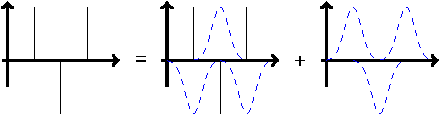
\includegraphics[width=0.9\textwidth]{figures/vmg_short-long-splitting.pdf}
\caption{The charge distribution consisting of point charges (left) is split into a smoothened part (right) and the rest (center), see~\vmgcite{1}}
\label{fig:vmg_long-short-splitting}
\end{figure}

In depth, the Coulomb problem is first split into a short-range and a long-range part, for when treated individually each can be solved efficiently. This is done by adding so-called shield charges at the same position as each point-like charge, see figure~\ref{fig:vmg_long-short-splitting}. These are described by a spline function that has compact support, is symmectric around its center and is normalized to the same magnitude as the original point-like charge. The short-range part (center,  fig.~\ref{fig:vmg_long-short-splitting}) is then solved by a direct summation of the pair-wise interactions between the small number of charges lying in the compact support of these shield charges. Outside of the support, shield charge and oppositely charged point-like charge precisely cancel. The long-range part consists of the potential induced by these shield charges. It is treated by solving a well-known partial differential equation (PDE) in the form $Lu=f$, the Poisson equation, where $L$ is the negated Laplace operator $L:=-\Delta$, $u$ is the sought-for solution and $f$ is the "right-hand side", i.\,e.~the shield charges sampled on the grid.

Solving PDEs numerically is usually done by discretizing their differential operator in an extension of the idea of calculating a derivative via the method of finite differences. This converts the continuous problem $Lu=f$ into a discrete problem $Ax=b$, where $A$ is the matrix of the discretized operator, $x$ is the discrete solution and $b$ is again the "right-hand side". In the multigrid ansatz, see~\vmgcite{2}, $Ax=b$ is obtained on the finest grid (of $d$ dimensions) while on coarser grids the so-called defect equation $Ax^\prime=b-Ax$ is solved. This offers the advantage that the solution time is independent of the system size. The basic idea of a multigrid is to eliminate the residual, i.\,e.~the error $(b-Ax)$, at each coarser and coarser level. The picture to have in mind is that the "noise" is reduced at multiple frequencies at the same time. 

A cycle of two grids, i.\,e.~a fine grid and a coarser one, then consists of steps of "removing noise" (smoothing), projecting down onto the coarser grid (restriction), solving exactly and bringing this solution back onto the finer grid (prolongation). A multigrid cycle then consists of the recursive application of two-grid cycles instead of solving exactly, i.\,e.~we step down the grid hierarchy from a finer to the next coarser grid and eventually move up again.

There are many types of this cycle differing in the precise sequence of smoothing, prolongation, and restriction steps. Since this is an iterative process we have to perform such a cycle a (typically small) number of times until the residual is small enough. Then we have "converged" sufficiently to the solution.

In order to set up the above PDE, we need the right-hand side $b$ that consists of the aforementioned shield charges. After solving the PDE on the grid, the Coulomb potential at the charge positions is obtained by some interpolation scheme. Right now, a multidimensional Newton interpolation is used, see \vmgcite{3}, where a polynomial is fit to the solution around the desired position. The field is calculated via analytical differentiation of these polynomials.

To sum it all up, the multigrid does the following:
\begin{enumerate}
 \item Bring the shield charges onto the grid (the right-hand side) by evaluating spline functions for each particle charge.
 \item Iterate over the multigrid in a specific cycle until either the (absolute or relative) residual is lower than a given threshold value (converged) or a set maximum number of iterations steps is reached (non-converged).
 \item The solution is interpolated back at the position of each charge, yielding the long-range interactions.
 \item Short-range interactions are determined via direct summation.
\end{enumerate}

Crucial for its accuracy are then the following parameters of the multigrid solver:
\begin{description}
 \item[grid size] This determines the number of grid points per axis on the finest level. This parameter mainly affects the accuracy of the long-range part of the solution.
 \item[width of spline support] This gives the width of the shield charges. The greater is the width, the more accurate the solution becomes, but at the same time the more interactions have to be evaluated with the (computationally expensive) short-range part of the solver. One has to ensure that the number of particles in the support of these shield charges is kept constant, otherwise the algorithm does not scale optimally anymore.
 \item[discretization scheme] This is the manner of constructing a matrix $A$ from the continuous Laplace operator $L$. A scheme of higher order gives greater accuracy w.r.t. a fixed grid size. This parameter is solely affecting the accuracy of the long-range part of the algorithm.
\end{description}

For parallelization the particles are distributed over many processes. Each brings its local particles onto the grid. Also, each process has a certain share of the grid and performs its multigrid operations on its share, communicating with neighboring processes during the restriction, prolongation, and smoothing. Conceptionally, there is also one global communication in every multigrid iteration where the local residuals get summed up globally. Eventually, each process interpolates back its particle potential.

\section*{Common capabilities}

\begin{description}

  \item[Periodicity:]
Currently only periodic boundary conditions are supported. Support for open or mixed boundary conditions is in progress.

  \item[Box shape:] Cubic boxes are supported.
  
  \item[Tolerances:] ?

  \item[Delegate near-field:] Not implemented.

  \item[Virial:] No.

\end{description}

\section*{Additional capabilities}

 Due to the aforementioned splitting of the Coulomb interactions into a short- and a long-range part, some parameters affect only the accuracy of either and not necessarily of both, see their desription. If then a system only has a small long-range part, one may save substantial calculation time by decreasing accuracy specifically for long-range calculations. This allows checking whether either interactions part far outweighs the other.
 Via the configure switch \emph{--enable-debug-output} the various energy contributions of short- and long-range parts are printed to the console. Note however that this switch should \emph{not be used for production runs} as it makes unnecessary additional calculations once an efficient set of parameters has been found.

% \begin{description}

% \end{description}

\section*{Solver specific functions}

\begin{itemize}

  \item
\begin{alltt}
fcs\_vmg\_set\_max\_level(FCS handle, fcs_int max_level);
\end{alltt}
Sets the number of points per axis of the finest grid (optional,default=6).
More specifically it is $2^{\text{max\_level}}$, i.e. more points means better approximated solution but scales with ${\cal O}(\text{max\_level}^3)$. This is the first value to change for better accuracy, see also near\_field\_cells.
  \item
\begin{alltt}
fcs\_vmg\_get\_max\_level(FCS handle, fcs\_int* max\_level);
\end{alltt}
Get the maximum level of the multigrid algorithm.

  \item
\begin{alltt}
fcs\_vmg\_set\_max\_iterations(FCS handle, fcs\_int max\_iterations);
\end{alltt}
Sets the maximum number of multigrid iterations (optional, default=15).
This is the second threshold besides \emph{precision} that will stop the iteration. Normally, you don't need to change this value, this is only present in case the iteration does not converge and this sets after how many iteration steps it is considered as "not converged".

  \item
\begin{alltt}
fcs\_vmg\_get\_max\_iterations(FCS handle, fcs\_int* max\_iterations);
\end{alltt}
Get the maximum number of multigrid iterations.

  \item
\begin{alltt}
fcs\_vmg\_set\_smoothing\_steps(FCS handle, fcs\_int smoothing\_steps);
\end{alltt}
Set the number of smoothing steps in the multigrid cycle per level (optional, default=3).
Smoothing refers to removal of error at a certain level. This is usually done for a fixed and small number of iterations. Usually, there is no need to change it. Fewer steps may be faster (and may cause solution not to converge anymore). Does not affect the precision but only the computational efficiency.

  \item
\begin{alltt}
fcs\_vmg\_get\_smoothing\_steps(FCS handle, fcs\_int *smoothing\_steps);
\end{alltt}
Get the number of pre/post-smoothing steps on each level.

  \item
\begin{alltt}
fcs\_vmg\_set\_cycle\_type(FCS handle, fcs\_int cycle\_type);
\end{alltt}
Specifies the type of multigrid cycle, 1 V-cycle, 2 W-cycle, \ldots (optional, default=1).
For parallel computation, V-cycle is the correct type, for serial computation W-cycle might be slightly more efficient. In case of doubt, leave it to default.

  \item
\begin{alltt}
fcs\_vmg\_get\_cycle\_type(FCS handle, fcs\_int *cycle\_type);
\end{alltt}
Get the cycle\_type-number of the multigrid cycle used.

  \item
\begin{alltt}
fcs\_vmg\_set\_precision(FCS handle, fcs\_float precision);
\end{alltt}
Set the threshold for (absolute and relative) residual below which internal iteration is stopped (optional, default=1.0e-8).
This is not equal to FCS's global tolerance! As an estimate one might use one magnitude below desired tolerance.

  \item
\begin{alltt}
fcs\_vmg\_get\_precision(FCS handle, fcs\_float *precision);
\end{alltt}

  \item
\begin{alltt}
fcs\_vmg\_set\_near\_field\_cells(FCS handle, fcs\_int near\_field\_cells);
\end{alltt}
Set the half witdh in number of grid points of compact local support of b-spline function (radius of shielding charges) (optional, default=4).
This value along with max\_level has great impact on accuracy but the correlation is reciprocal.

  \item
\begin{alltt}
fcs\_vmg\_get\_near\_field\_cells(FCS handle, fcs\_int *near\_field\_cells);
\end{alltt}
Get the number of near field cells for separating the near/far field part of the potential.

  \item
\begin{alltt}
fcs\_vmg\_set\_interpolation\_order(FCS handle, fcs\_int interpolation\_order);
\end{alltt}
Set polynomial order of tensored Newton back-interpolation of solution at the site of each charge (optional, default=5).
Usually, does not need to be changed. Normally, less means precision of grid solution is omitted, more means useless computation.

  \item
\begin{alltt}
fcs\_vmg\_get\_interpolation\_order(FCS handle, fcs\_int *interpolation\_order);
\end{alltt}
Get the interpolation order for interpolating the gridded potential to the particle positions.

  \item
\begin{alltt}
fcs\_vmg\_set\_discretization\_order(FCS handle, fcs\_int discretization\_order);
\end{alltt}
Discretization scheme in setting up partial differential equation (optional, [2,4], default=4).
This heavily influences precision of solution in conjunction with near\_field\_cells ans max\_level. This parameter enables direct control of the discretization error of the long-range part. Default is 4 and leave it at that.

  \item
\begin{alltt}
fcs\_vmg\_get\_discretization\_order(FCS handle, fcs\_int *discretization\_order);
\end{alltt}
Get the order of the discretization scheme.

\end{itemize}

\section*{Known bugs or missing features}

\begin{itemize}
  \item Open and mixed boundaries still need to be incorporated.
  \item Separate near-field part?
  \item How to compute the virial?
\end{itemize}

\paragraph{References}
\todo[inline]{move vmg citations to bibliography}
\begin{footnotesize}
\begin{itemize}
  \item[vmg-1] M.~Griebel, S.~Knapek, G.~Zumbusch \textbf{Numerical Simulation in Molecular Dynamics -- Numerics, Algorithms, Parallelization, Applications}, 2007
  \item[vmg-2] U.~Trottenberg, C.~W.~Oosterlee, A.~Schuller \textbf{Multigrid}, 2000
  \item[vmg-3] K.~A.~Atkinson \textbf{Introduction to Numerical Analysis}, 1988
\end{itemize}
\end{footnotesize}


%%% Local Variables: 
%%% mode: latex
%%% TeX-master: ug.tex
%%% End: 


%%% Local Variables: 
%%% mode: latex
%%% TeX-master: ug.tex
%%% End: 


\chapter{direct -- Direct summation}
\label{cha:direct}

\solvertoindex{direct}
\solvertoindex{Direct Summation}

The direct solver implemented within the ScaFaCoS library performs a direct summation of the pair-wise interactions between all given particles.
The parallel computations use the given distribution of particles among parallel MPI processes (i.e., no additional redistribution for improving the load-balancing is performed).
Let $p$ be the number of parallel MPI processes.
After each process has computed the interactions between its local particles, $p-1$ steps are performed to compute interactions with all non-local particles.
In each step, each process receives the particles of the preceding process, computes the interactions with its local particles, and sends to the previously received particles to the succeeding process.

\section*{Common capabilities}

\begin{description}

  \item[Periodicity:]
Open, periodic, or mixed boundaries are supported.
The box shape is not limited by the chosen periodicity.
Periodic boundaries are computed by placing a number of periodic images of the particle system around the given particle system.
The number of images to use in each (periodic) dimensions can be specified with \texttt{fcs\_direct\_set\_periodic\_images}.

  \item[Box shape:] Any (triclinic) box shape is supported.
  
  \item[Tolerances:] No.

  \item[Delegate near-field:] No.

  \item[Virial:] ?

\end{description}

\section*{Additional capabilities}

\begin{description}

  \item[Cutoff:]
\texttt{fcs\_direct\_set\_cutoff} can be used to specify a cutoff range that limits the computation of interactions.
If the cutoff range is 0, then all interactions are considered.
If the cutoff range is greater than 0, then only interactions inside the cufoff range are considered.
If the cutoff range is less than 0, then only interactions outside the (positive) cufoff range are considered.
If the cutoff range is greater than 0, then \texttt{fcs\_direct\_set\_cutoff\_with\_near} can be used to enable the ScaFaCoS internal near-field solver module instead of the direct solver.

\end{description}

\section*{Solver specific functions}

\begin{itemize}

  \item
\begin{alltt}
fcs\_direct\_set\_cutoff(FCS handle, fcs_float cutoff);
\end{alltt}
Set the current cutoff range (optional, default = 0).

  \item
\begin{alltt}
fcs_direct_get_cutoff(FCS handle, fcs_float *cutoff);
\end{alltt}
Retrieve the current cutoff range.

  \item
\begin{alltt}
fcs_direct_set_periodic_images(FCS handle, fcs_int *periodic_images);
\end{alltt}
Set the number of periodic images to use for computations with periodic boundaries (optional, default = \{ 1, 1, 1 \}).

  \item
\begin{alltt}
fcs_direct_get_periodic_images(FCS handle, fcs_int *periodic_images);
\end{alltt}
Retrieve the number of periodic images used for computations with periodic boundaries.

  \item
\begin{alltt}
fcs_direct_set_cutoff_with_near(FCS handle, fcs_bool cutoff_with_near);
\end{alltt}
Enable the near-field solver module (instead of the direct solver) to be used for computations with a cutoff range.

  \item
\begin{alltt}
fcs_direct_get_cutoff_with_near(FCS handle, fcs_bool *cutoff_with_near);
\end{alltt}
Retrieve whether the near-field solver module is used for computations with a cutoff range.

\end{itemize}

\section*{Known bugs or missing features}

\begin{itemize}
  \item Periodic boundaries still need to be tested.
  \item How to compute the virial for periodic boundaries?
\end{itemize}

%%% Local Variables: 
%%% mode: latex
%%% TeX-master: ug.tex
%%% End: 

\chapter{List of Functions}
\label{cha:appendix_function_list}

This chapter lists all the functions within the ScaFaCoS interface, which can be used by the user to manipulate the library.

\section{Mandatory Functions}
\begin{figure}[htb]
\begin{lstlisting}[language=C,frame=trBL,breaklines,basicstyle=\ttfamily]
/* C */
FCSResult fcs_init(FCS handle, char* method, MPI_Comm comm);
\end{lstlisting}
\begin{lstlisting}[language=Fortran,frame=trBL,breaklines,basicstyle=\ttfamily]
! Fortran
function fcs_init(handle,method,comm)
type(c_ptr)                                 :: handle
char                                        :: method(*)
integer(kind = c_int)                       :: comm
type(c_ptr)                                 :: fcs_init
\end{lstlisting}
\caption{Function call: fcs\_init}
\label{fig:fcs_init}
\ufunctiontoindex{fcs\_init}
\end{figure}
\begin{figure}[htb]
\begin{lstlisting}[language=C,frame=trBL,breaklines,basicstyle=\ttfamily,prebreak={\raisebox{0ex}[0ex][0ex]{\ensuremath{\hookleftarrow}}}]
/* C */
FCSResult fcs_set_common(FCS handle, fcs_int short_range_flag, fcs_float* box_a, fcs_float* box_b, fcs_float* box_c, fcs_float* offset, fcs_int* periodicity, fcs_int total_particles);
\end{lstlisting}
\begin{lstlisting}[language=Fortran,frame=trBL,breaklines,basicstyle=\ttfamily,prebreak={\raisebox{0ex}[0ex][0ex]{\ensuremath{\hookleftarrow}}}]
! Fortran
function fcs_set_common(handle,short_range_flag,box_a,box_b,box_c,offset,periodicity,total_particles)
type(c_ptr)                                 ::  handle
logical                                     ::  short_range_flag
real(kind = fcs_real_kind_isoc)             ::  box_a(3)
real(kind = fcs_real_kind_isoc)             ::  box_b(3)
real(kind = fcs_real_kind_isoc)             ::  box_c(3)
real(kind = fcs_real_kind_isoc)             ::  offset(3)
logical                                     ::  periodicity(3)
integer(kind = fcs_integer_kind_isoc)       ::  total_parts
type(c_ptr)                                 ::  fcs_set_common
\end{lstlisting}
\caption{Function call: fcs\_common\_set}
\label{fig:fcs_set_common}
\ufunctiontoindex{fcs\_common\_set}
\end{figure}
\begin{figure}[htb]
\begin{lstlisting}[language=C,frame=trBL,breaklines,basicstyle=\ttfamily,prebreak={\raisebox{0ex}[0ex][0ex]{\ensuremath{\hookleftarrow}}}]
/* C */
FCSResult fcs_tune (FCS handle, fcs_int local_particles, fcs_int local_max_particles, fcs_float *positions, fcs_float *charges);
\end{lstlisting}
\begin{lstlisting}[language=Fortran,frame=trBL,breaklines,basicstyle=\ttfamily,prebreak={\raisebox{0ex}[0ex][0ex]{\ensuremath{\hookleftarrow}}}]
! Fortran
function fcs_tune(handle,n_locp,n_maxlocp,positions,charges)
type(c_ptr), value                          :: handle
integer(kind = fcs_integer_kind_isoc),value :: n_locp
integer(kind = fcs_integer_kind_isoc),value :: n_maxlocp
real(kind = fcs_real_kind_isoc)             :: positions(3*n_locp)
real(kind = fcs_real_kind_isoc)             :: charges(n_locp)
type(c_ptr)                                 :: fcs_tune
\end{lstlisting}
\caption{Function call: fcs\_tune}
\label{fig:fcs_tune}
\ufunctiontoindex{fcs\_tune}
\end{figure}
\begin{figure}[htb]
\begin{lstlisting}[language=C,frame=trBL,breaklines,basicstyle=\ttfamily,prebreak={\raisebox{0ex}[0ex][0ex]{\ensuremath{\hookleftarrow}}}]
/* C */
FCSResult fcs_run (FCS handle, fcs_int local_particles, fcs_int local_max_particles, fcs_float *positions, fcs_float *charges, fcs_float *field, fcs_float *potentials);
\end{lstlisting}
\begin{lstlisting}[language=Fortran,frame=trBL,breaklines,basicstyle=\ttfamily,prebreak={\raisebox{0ex}[0ex][0ex]{\ensuremath{\hookleftarrow}}}]
! Fortran
function fcs_run(handle,n_locp,n_maxlocp,positions,charges,field,potential)
type(c_ptr), value                          :: handle
integer(kind = fcs_integer_kind_isoc),value :: n_locp
integer(kind = fcs_integer_kind_isoc),value :: n_maxlocp
real(kind = fcs_real_kind_isoc)             :: positions(3*n_locp)
real(kind = fcs_real_kind_isoc)             :: charges(n_locp)
real(kind = fcs_real_kind_isoc)             :: field(3*n_locp)
real(kind = fcs_real_kind_isoc)             :: potential(n_locp)
type(c_ptr)                                 :: fcs_run
\end{lstlisting}
\caption{Function call: fcs\_run}
\label{fig:fcs_run}
\ufunctiontoindex{fcs\_run}
\end{figure}
\begin{figure}[htb]
\begin{lstlisting}[language=C,frame=trBL,breaklines,basicstyle=\ttfamily,prebreak={\raisebox{0ex}[0ex][0ex]{\ensuremath{\hookleftarrow}}}]
/* C */
FCSResult fcs_destroy (FCS handle);
\end{lstlisting}
\begin{lstlisting}[language=Fortran,frame=trBL,breaklines,basicstyle=\ttfamily,prebreak={\raisebox{0ex}[0ex][0ex]{\ensuremath{\hookleftarrow}}}]
! Fortran
function fcs_destroy(handle)
type(c_ptr), value                          :: handle
type(c_ptr)                                 :: fcs_run
\end{lstlisting}
\caption{Function call: fcs\_destroy}
\label{fig:fcs_destroy}
\ufunctiontoindex{fcs\_destroy}
\end{figure}
\FloatBarrier
\section{Generic Functions}

\FloatBarrier
\subsection{Errorhandling}

\begin{figure}[htb]
\begin{lstlisting}[language=C,frame=trBL,breaklines,basicstyle=\ttfamily,prebreak={\raisebox{0ex}[0ex][0ex]{\ensuremath{\hookleftarrow}}}]
/* C */
fcs_int fcsResult_getReturnCode (FCSResult err);
\end{lstlisting}
\begin{lstlisting}[language=Fortran,frame=trBL,breaklines,basicstyle=\ttfamily,prebreak={\raisebox{0ex}[0ex][0ex]{\ensuremath{\hookleftarrow}}}]
! Fortran
function fcsResult_getReturnCode(res)
type(c_ptr)                            ::  res
integer(kind = fcs_integer_kind_isoc)  ::  fcsResult_getReturnCode
\end{lstlisting}
\caption{Function call: fcsResult\_getReturnCode}
\label{fig:fcsResult_getReturnCode}
\ufunctiontoindex{fcsResult\_getReturnCode}
\end{figure}

\begin{figure}[htb]
\begin{lstlisting}[language=C,frame=trBL,breaklines,basicstyle=\ttfamily,prebreak={\raisebox{0ex}[0ex][0ex]{\ensuremath{\hookleftarrow}}}]
/* C */
const char* fcsResult_getErrorMessage (FCSResult err);
\end{lstlisting}
\begin{lstlisting}[language=Fortran,frame=trBL,breaklines,basicstyle=\ttfamily,prebreak={\raisebox{0ex}[0ex][0ex]{\ensuremath{\hookleftarrow}}}]
! Fortran
function fcsResult_getErrorMessage(res)
type(c_ptr)                                     ::  res
character(kind = c_char, len = MESSAGE_LENGTH)  ::  fcsResult_getErrorMessage
\end{lstlisting}
\caption{Function call: fcsResult\_getErrorMessage}
\label{fig:fcsResult_getErrorMessage}
\ufunctiontoindex{fcsResult\_getErrorMessage}
\end{figure}

\begin{figure}[htb]
\begin{lstlisting}[language=C,frame=trBL,breaklines,basicstyle=\ttfamily,prebreak={\raisebox{0ex}[0ex][0ex]{\ensuremath{\hookleftarrow}}}]
/* C */
const char* fcsResult_getErrorSource (FCSResult err);
\end{lstlisting}
\begin{lstlisting}[language=Fortran,frame=trBL,breaklines,basicstyle=\ttfamily,prebreak={\raisebox{0ex}[0ex][0ex]{\ensuremath{\hookleftarrow}}}]
! Fortran
function fcsResult_getErrorSource(res)
type(c_ptr)                                     ::  res
character(kind = c_char, len = MESSAGE_LENGTH)  ::  fcsResult_getErrorSource
\end{lstlisting}
\caption{Function call: fcsResult\_getErrorSource}
\label{fig:fcsResult_getErrorSource}
\ufunctiontoindex{fcsResult\_getErrorSource}
\end{figure}

\FloatBarrier
\subsection{Getters and Setters}



\FloatBarrier
\subsection{Near Field Computations}

\begin{figure}[htb]
\begin{lstlisting}[language=C,frame=trBL,breaklines,basicstyle=\ttfamily,prebreak={\raisebox{0ex}[0ex][0ex]{\ensuremath{\hookleftarrow}}}]
/* C */
FCSResult fcs_compute_near_field (FCS handle, fcs_float dist, fcs_float *field);
\end{lstlisting}
\begin{lstlisting}[language=Fortran,frame=trBL,breaklines,basicstyle=\ttfamily,prebreak={\raisebox{0ex}[0ex][0ex]{\ensuremath{\hookleftarrow}}}]
! Fortran
function fcs_compute_near_field(handle,dist,field)
type(c_ptr)                                     ::  handle
real(kind = fcs_real_kind_isoc)                 ::  dist
real(kind = fcs_real_kind_isoc), dimension(3)   ::  field
type(c_ptr)                                     ::  fcs_compute_near_field
\end{lstlisting}
\caption{Function call: fcs\_compute\_near\_field}
\label{fig:fcs_compute_near_field}
\ufunctiontoindex{fcs\_compute\_near\_field}
\end{figure}

\begin{figure}[htb]
\begin{lstlisting}[language=C,frame=trBL,breaklines,basicstyle=\ttfamily,prebreak={\raisebox{0ex}[0ex][0ex]{\ensuremath{\hookleftarrow}}}]
/* C */
FCSResult fcs_compute_near_potential (FCS handle, fcs_float dist, fcs_float *pot);
\end{lstlisting}
\begin{lstlisting}[language=Fortran,frame=trBL,breaklines,basicstyle=\ttfamily,prebreak={\raisebox{0ex}[0ex][0ex]{\ensuremath{\hookleftarrow}}}]
! Fortran
function fcs_compute_near_potential(handle,dist,pot)
type(c_ptr)                                     ::  handle
real(kind = fcs_real_kind_isoc)                 ::  dist
real(kind = fcs_real_kind_isoc)                 ::  pot
type(c_ptr)                                     ::  fcs_compute_near_potential
\end{lstlisting}
\caption{Function call: fcs\_compute\_near\_potential}
\label{fig:fcs_compute_near_potential}
\ufunctiontoindex{fcs\_compute\_near\_potential}
\end{figure}

\begin{figure}[htb]
\begin{lstlisting}[language=C,frame=trBL,breaklines,basicstyle=\ttfamily,prebreak={\raisebox{0ex}[0ex][0ex]{\ensuremath{\hookleftarrow}}}]
/* C */
FCSResult fcs_compute_near (FCS handle, fcs_float dist, fcs_float *pot, fcs_float *field);
\end{lstlisting}
\begin{lstlisting}[language=Fortran,frame=trBL,breaklines,basicstyle=\ttfamily,prebreak={\raisebox{0ex}[0ex][0ex]{\ensuremath{\hookleftarrow}}}]
! Fortran
function fcs_compute_near(handle,dist,pot,field)
type(c_ptr)                                     ::  handle
real(kind = fcs_real_kind_isoc)                 ::  dist
real(kind = fcs_real_kind_isoc)                 ::  pot
real(kind = fcs_real_kind_isoc), dimension(3)   ::  field
type(c_ptr)                                     ::  fcs_compute_near
\end{lstlisting}
\caption{Function call: fcs\_compute\_near}
\label{fig:fcs_compute_near}
\ufunctiontoindex{fcs\_compute\_near}
\end{figure}

\begin{figure}[htb]
\begin{lstlisting}[language=C,frame=trBL,breaklines,basicstyle=\ttfamily,prebreak={\raisebox{0ex}[0ex][0ex]{\ensuremath{\hookleftarrow}}}]
/* C */
FCSResult fcs_method_has_near (FCS handle, fcs_int *has_near);
\end{lstlisting}
\begin{lstlisting}[language=Fortran,frame=trBL,breaklines,basicstyle=\ttfamily,prebreak={\raisebox{0ex}[0ex][0ex]{\ensuremath{\hookleftarrow}}}]
! Fortran
function fcs_method_has_near(handle,has_near)
type(c_ptr)                                     ::  handle
real(kind = fcs_real_kind_isoc)                 ::  dist
real(kind = fcs_real_kind_isoc), dimension(3)   ::  field
type(c_ptr)                                     ::  fcs_compute_near_field
\end{lstlisting}
\caption{Function call: fcs\_method\_has\_near}
\label{fig:fcs_method_has_near}
\ufunctiontoindex{fcs\_method\_has\_near}
\end{figure}

\todo{fcs\_method\_has\_near fehlt!}

\FloatBarrier
\subsection{Output}

\begin{figure}[htb]
\begin{lstlisting}[language=C,frame=trBL,breaklines,basicstyle=\ttfamily,prebreak={\raisebox{0ex}[0ex][0ex]{\ensuremath{\hookleftarrow}}}]
/* C */
void fcs_printHandle (FCS handle);
\end{lstlisting}
\begin{lstlisting}[language=Fortran,frame=trBL,breaklines,basicstyle=\ttfamily,prebreak={\raisebox{0ex}[0ex][0ex]{\ensuremath{\hookleftarrow}}}]
! Fortran
subroutine fcs_printHandle(handle)
type(c_ptr)                                     ::  handle
\end{lstlisting}
\caption{Function call: fcs\_printHandle}
\label{fig:fcs_printHandle}
\ufunctiontoindex{fcs\_printHandle}
\end{figure}


\FloatBarrier
\subsection{Parser}

\begin{figure}[htb]
\begin{lstlisting}[language=C,frame=trBL,breaklines,basicstyle=\ttfamily,prebreak={\raisebox{0ex}[0ex][0ex]{\ensuremath{\hookleftarrow}}}]
/* C */
FCSResult fcs_parser (FCS handle, const char* parse_string);
\end{lstlisting}
\begin{lstlisting}[language=Fortran,frame=trBL,breaklines,basicstyle=\ttfamily,prebreak={\raisebox{0ex}[0ex][0ex]{\ensuremath{\hookleftarrow}}}]
! Fortran
function fcs_printHandle(handle,parse_string)
type(c_ptr)                                     ::  handle
character(kind = c_char, len = *)               ::  parse_string
type(c_ptr)                                     ::  fcs_parser
\end{lstlisting}
\caption{Function call: fcs\_parser}
\label{fig:fcs_parser}
\ufunctiontoindex{fcs\_parser}
\end{figure}

\FloatBarrier
\subsection{Virial}

\begin{figure}[htb]
\begin{lstlisting}[language=C,frame=trBL,breaklines,basicstyle=\ttfamily,prebreak={\raisebox{0ex}[0ex][0ex]{\ensuremath{\hookleftarrow}}}]
/* C */
FCSResult fcs_require_virial (FCS handle, fcs_int flag);
\end{lstlisting}
\begin{lstlisting}[language=Fortran,frame=trBL,breaklines,basicstyle=\ttfamily,prebreak={\raisebox{0ex}[0ex][0ex]{\ensuremath{\hookleftarrow}}}]
! Fortran
function fcs_require_virial(handle,flag)
type(c_ptr)                                     ::  handle
logical                                         ::  dist
type(c_ptr)                                     ::  fcs_require_virial
\end{lstlisting}
\caption{Function call: fcs\_require\_virial}
\label{fig:fcs_require_virial}
\ufunctiontoindex{fcs\_require\_virial}
\end{figure}

\begin{figure}[htb]
\begin{lstlisting}[language=C,frame=trBL,breaklines,basicstyle=\ttfamily,prebreak={\raisebox{0ex}[0ex][0ex]{\ensuremath{\hookleftarrow}}}]
/* C */
FCSResult fcs_get_virial (FCS handle, fcs_float* virial);
\end{lstlisting}
\begin{lstlisting}[language=Fortran,frame=trBL,breaklines,basicstyle=\ttfamily,prebreak={\raisebox{0ex}[0ex][0ex]{\ensuremath{\hookleftarrow}}}]
! Fortran
function fcs_get_virial(handle,virial)
type(c_ptr)                                     ::  handle
real(kind = fcs_real_kind_isoc), dimension(9)   ::  dist
type(c_ptr)                                     ::  fcs_require_virial
\end{lstlisting}
\caption{Function call: fcs\_get\_virial}
\label{fig:fcs_get_virial}
\ufunctiontoindex{fcs\_get\_virial}
\end{figure}

\FloatBarrier
\section{Direct Solver specific Functions}


\FloatBarrier
\subsection{Getters and Setters}

\FloatBarrier
\section{Ewald Solver specific Functions}


\FloatBarrier
\subsection{Getters and Setters}

\FloatBarrier
\section{FMM Solver specific Functions}


\FloatBarrier
\subsection{Getters and Setters}

\FloatBarrier
\section{MEMD Solver specific Functions}


\FloatBarrier
\subsection{Getters and Setters}

\FloatBarrier
\section{MMM1D Solver specific Functions}


\FloatBarrier
\subsection{Getters and Setters}

\FloatBarrier
\section{MMM2D Solver specific Functions}


\FloatBarrier
\subsection{Getters and Setters}

\FloatBarrier
\section{PEPC Solver specific Functions}


\FloatBarrier
\subsection{Getters and Setters}

\FloatBarrier
\section{PP3MG Solver specific Functions}


\FloatBarrier
\subsection{Getters and Setters}

\FloatBarrier
\section{P2NFFT Solver specific Functions}


\FloatBarrier
\subsection{Getters and Setters}

\FloatBarrier
\section{P3M Solver specific Functions}

\FloatBarrier
\subsection{Getters and Setters}

\FloatBarrier
\subsection{Near Field Computations}

\begin{figure}[htb]
\begin{lstlisting}[language=C,frame=trBL,breaklines,basicstyle=\ttfamily,prebreak={\raisebox{0ex}[0ex][0ex]{\ensuremath{\hookleftarrow}}}]
/* C */
FCSResult fcs_p3m_compute_near_field (FCS handle, fcs_float dist, fcs_float *field);
\end{lstlisting}
\begin{lstlisting}[language=Fortran,frame=trBL,breaklines,basicstyle=\ttfamily,prebreak={\raisebox{0ex}[0ex][0ex]{\ensuremath{\hookleftarrow}}}]
! Fortran
function fcs_p3m_compute_near_field(handle,dist,field)
type(c_ptr)                                     ::  handle
real(kind = fcs_real_kind_isoc)                 ::  dist
real(kind = fcs_real_kind_isoc), dimension(3)   ::  field
type(c_ptr)                                     ::  fcs_p3m_compute_near_field
\end{lstlisting}
\caption{Function call: fcs\_p3m\_compute\_near\_field}
\label{fig:fcs_p3m_compute_near_field}
\ufunctiontoindex{fcs\_p3m\_compute\_near\_field}
\end{figure}

\begin{figure}[htb]
\begin{lstlisting}[language=C,frame=trBL,breaklines,basicstyle=\ttfamily,prebreak={\raisebox{0ex}[0ex][0ex]{\ensuremath{\hookleftarrow}}}]
/* C */
FCSResult fcs_p3m_compute_near_potential (FCS handle, fcs_float dist, fcs_float *pot);
\end{lstlisting}
\begin{lstlisting}[language=Fortran,frame=trBL,breaklines,basicstyle=\ttfamily,prebreak={\raisebox{0ex}[0ex][0ex]{\ensuremath{\hookleftarrow}}}]
! Fortran
function fcs_p3m_compute_near_potential(handle,dist,pot)
type(c_ptr)                                     ::  handle
real(kind = fcs_real_kind_isoc)                 ::  dist
real(kind = fcs_real_kind_isoc)                 ::  pot
type(c_ptr)                                     ::  fcs_p3m_compute_near_potential
\end{lstlisting}
\caption{Function call: fcs\_p3m\_compute\_near\_potential}
\label{fig:fcs_p3m_compute_near_potential}
\ufunctiontoindex{fcs\_p3m\_compute\_near\_potential}
\end{figure}

\begin{figure}[htb]
\begin{lstlisting}[language=C,frame=trBL,breaklines,basicstyle=\ttfamily,prebreak={\raisebox{0ex}[0ex][0ex]{\ensuremath{\hookleftarrow}}}]
/* C */
FCSResult fcs_p3m_compute_near (FCS handle, fcs_float dist, fcs_float *pot, fcs_float *field);
\end{lstlisting}
\begin{lstlisting}[language=Fortran,frame=trBL,breaklines,basicstyle=\ttfamily,prebreak={\raisebox{0ex}[0ex][0ex]{\ensuremath{\hookleftarrow}}}]
! Fortran
function fcs_p3m_compute_near(handle,dist,pot,field)
type(c_ptr)                                     ::  handle
real(kind = fcs_real_kind_isoc)                 ::  dist
real(kind = fcs_real_kind_isoc)                 ::  pot
real(kind = fcs_real_kind_isoc), dimension(3)   ::  field
type(c_ptr)                                     ::  fcs_p3m_compute_near
\end{lstlisting}
\caption{Function call: fcs\_p3m\_compute\_near}
\label{fig:fcs_p3m_compute_near}
\ufunctiontoindex{fcs\_p3m\_compute\_near}
\end{figure}

\FloatBarrier
\section{VMG Solver specific Functions}

\FloatBarrier
%%% Local Variables: 
%%% mode: latex
%%% TeX-master: ug.tex
%%% End: 


\part{Developer's Guide}
\chapter{Build System}
\label{cha:buildsystem}
\index{Build System}

\begin{verbatim}
Prerequisites
-------------

This source tree uses GNU autotools
<http://www.gnu.org/software/automake/manual/html_node/Autotools-Introduction.html>

In order to do development, please make sure you have reasonably recent
versions of the following tools installed and in your $PATH:
  GNU m4       >= 1.4.13  http://ftp.gnu.org/gnu/m4/m4-1.4.16.tar.gz
  GNU Autoconf >= 2.64    http://ftp.gnu.org/gnu/autoconf/autoconf-2.68.tar.gz
  GNU Automake >= 1.11    http://ftp.gnu.org/gnu/automake/automake-1.11.3.tar.gz
  GNU Libtool  >= 2.2.6b  http://ftp.gnu.org/gnu/libtool/libtool-2.4.2.tar.gz

Then, set up the autotools infrastructure:
  ./bootstrap

This should create configure, Makefile.in, and config.h.in files.

If that went without trouble, continue as described in the README file.
\end{verbatim}

To learn how to install the Autotools, have a look at
\url{http://www.gnu.org/software/automake/faq/autotools-faq.html#How-do-I-install-the-Autotools-_0028as-user_0029_003f}.

\begin{verbatim}
Build system layout
-------------------

There is a toplevel configure.ac script and helper macros in the m4/
subdirectory.  Each directory where stuff needs to be done later gets
a Makefile.am file which is processed by automake and later by configure.

In order to facilitate modularity of the different solver methods, each
method gets its own configure.ac script in libs/$method/ as well.  The
toplevel configure will call each of the lower-level ones which are
enabled and present in turn.

The generated makefiles support all of the standard targets described here:
<http://www.gnu.org/software/automake/manual/html_node/Standard-Targets.html>


Generated files
---------------

The autotools build system uses several generated files and a few helper
scripts:

1) Helper scripts installed below build-aux/ subdirectories:
- depcomp
- install-sh
- compile
- missing

2a) File generated at bootstrap time, and distributed to end-users:
- aclocal.m4      macro files generated by aclocal
- configure       scripts are generated from configure.ac files and additional
                  macro files (aclocal.m4 and files in some m4/ subdirectory)
- Makefile.in     template files generated by automake (and later converted to
                  Makefile files by config.status)
- config.h.in     header template file generated by autoheader (and later
                  converted to config.h by config.status)

2b) File generated at bootstrap time, NOT distributed to end-users:
- autom4te.cache  directory containing autotools-internal cache files.
                  This may be safely removed at any time.

3) Files generated at configure run time by the end-user:
- config.log      a log file containing detailed configure test results
- config.status   a script file containing the test results
- config.cache    a cache of test results (used when --config-cache is given)
- Makefile        the actual makefiles generated by config.status
- config.h        a project-specific header that should not be installed
- .deps/*         dependency tracking makefile snippets
- stamp-*          makefile stamp files

and of course object files and programs etc.

None of these files should be committed to SVN, because the files in (1) and
in (2) may differ between different autotools versions (causing spurious
differences with "svn diff" when two developers use different versions)
and because the files in (3) are system-dependent.

For further reading see:
<http://www.gnu.org/software/autoconf/manual/html_node/Making-configure-Scripts.html>
<http://www.gnu.org/software/automake/manual/html_node/CVS.html>

How to add a new solver
-----------------------

If you are adding a new solver to the build system, please adjust the
following build system files:

- Either convert your build system below lib/SOLVER to autotools or ensure
  that the usual GNU targets are supported by your makefiles and that VPATH
  building works; see here for more information:
  <http://www.gnu.org/software/automake/manual/html_node/Third_002dParty-Makefiles.html>
  <http://www.gnu.org/software/automake/manual/html_node/Standard-Targets.html>

- Add your solver to the toplevel all_solver_methods macro in the toplevel
  configure.ac script.  If your solver contains GPL code, or relies on GPL
  libraries, add your solver to the gpl_solver_methods macro in the toplevel
  configure.ac script.  Add the list of libraries the user should link to
  to the SCAFACOS_LIBS variable near the end of the script.

- Document in the toplevel README any required libraries for your solver.

- For each Makefile.am you add,
  - adjust the SUBDIRS line in the next-higher Makefile.am file,
  - add an 'AC_CONFIG_FILES([.../Makefile])' line to the next-higher
    configure.ac, with the correct relative path.

- In each Makefile.am file that deals with preprocessed Fortran, add
    include $(top_srcdir)/build-aux/fortran-rules.am

  to ensure .f90 files are preprocessed.

- For each C, C++ source file, add
    #ifdef HAVE_CONFIG_H
    #include <config.h>
    #endif

  before the first included header.  However, do not add this to header
  files, esp. not to header files that are installed later.
  (Note that end-users of scafacos-fcs like IMD should instead include
  an installed header like fcs.h.)

- For preprocessed Fortran source file in a method, add
    #ifdef HAVE_FCONFIG_H
    #include <fconfig.h>
    #endif

  before the first included header.

- In the toplevel fconfig.h.in file, add the following lines for your solver:
    ! Whether solver method <solver> is enabled.
    #undef FCS_ENABLE_<SOLVER>

- Ensure src and test are adjusted (FIXME: please elaborate here)

- Finally, rerun ./bootstrap in the toplevel source directory, then proceed
  as described in README.
\end{verbatim}
%%% Local Variables: 
%%% mode: latex
%%% TeX-master: ug.tex
%%% End: 

\chapter{Implementation}
\label{cha:implementation}

\index{Implementation}

\section{Licenses}
\label{sec:licenses}

\subsection{Applying the (L)GPL}

To apply the (L)GPL to your program, do the following:

\begin{itemize}
\item Add the following header text in a comment to all of your files
  (source files and text files!):

\begin{verbatim}
  Copyright (C) 2011 <authors>

  This file is part of ScaFaCoS.

  ScaFaCoS is free software: you can redistribute it and/or modify it
  under the terms of the GNU Lesser Public License as published by the
  Free Software Foundation, either version 3 of the License, or (at
  your option) any later version.

  ScaFaCoS is distributed in the hope that it will be useful, but
  WITHOUT ANY WARRANTY; without even the implied warranty of
  MERCHANTABILITY or FITNESS FOR A PARTICULAR PURPOSE.  See the GNU
  Lesser Public License for more details.

  You should have received a copy of the GNU Lesser Public License
  along with this program.  If not, see
  <http://www.gnu.org/licenses/>.
\end{verbatim}

\item Replace the word \texttt{<authors>} with the names of the
  authors that have written the file.  If you want to use the GPL
  instead of the LGPL, replace the word \textit{Lesser} in the text by
  \textit{General} in all three places.
\end{itemize}

\subsection{Simple files}

For simple files, you might prefer not to use the long header of the
(L)GPL, instead you can use:

\begin{verbatim}
Copyright (C) 2011 <authors>

Copying and distribution of this file, with or without modification,
are permitted in any medium without royalty provided the copyright
notice and this notice are preserved.  This file is offered as-is,
without any warranty.
\end{verbatim}

\chapter{Test Environment}
\label{cha:tests}

\newcommand{\gentestexec}{scafacos\_test}
\newcommand{\gentestdir}{tests/generic}

\section{Generic Test Program \texttt{\gentestexec}}

\noindent
The generic test program \texttt{\gentestexec} located in \texttt{\gentestdir} can be used to perform precision and performance tests with all solver methods in a common way.
The test case to be computed has to specified in form of an \emph{XML file}.
A single XML file can contain several particle configurations to be computed one after another using the same solver method.
The particle data (i.e., position and charge values as well as optional potential and field reference values) can either be read from the input file(s) (plain text or binary format) or generated \emph{online} using several internal particle data generators.
Furthermore, the particle system(s) to be computed can explicitly increased by duplicating the given input particles several times.
Additionally, the test program can write the result of the computations to a new XML output file.
This can be used to create potential and field reference values using one of the implemented solvers as reference method.

\subsubsection*{Usage:}

\begin{alltt}
  ./\gentestexec [OPTIONS] METHOD FILE
\end{alltt}

\noindent
The test program has to be executed in parallel using MPI (e.g. with \texttt{mpiexec -n NUMPROCS ./\gentestexec ...}).
\texttt{METHOD} specifies the solver method to be used and can be any method name supported by the FCS init function \texttt{fcs\_init} (see \ref{sec:init_step}).
Additionally, the method name can also be \texttt{none} to pass the test case through the test program (including parsing, particle data generation, duplication, and output), but without executing a solver.
\texttt{FILE} specifies the XML file describing the test case to be computed.
If the zlib compression library was available during building the library, then the XML files can also be compressed.
The command line arguments are only read on the master process.

\subsubsection*{Options:}

\noindent
The given command line arguments override conflicting settings that may already exist within the XML file that specifies the test case.

\begin{tabular}{lp{0.8\textwidth}}

\texttt{-o OUTFILE} &
Write the given test case including the computed results to a new XML file \texttt{OUTFILE}.
\\
\texttt{-b} &
Write the particle data in a machine-dependent binary format to a separate file (basename of \texttt{OUTFILE} with 'bin' suffix.
This is only useful together with \texttt{-o} option.
\\
\texttt{-d DUP} &
Duplicate a given periodic particle system in each \emph{periodic} dimension.
\texttt{DUP} can be a single value X or three values XxYxZ (i.e., one separate value for each dimension).
The default value of \texttt{DUP} = 1 is equivalent to no duplication.
\\
\texttt{-m MODE} &
Specify how the input particle data is distributed among parallel processes before the solver is executed.
Mode can be one of the following:
\begin{compactitem}
  \item \texttt{atomistic}: Equal distribution without any further assumptions (this is the \emph{default}).
  \item \texttt{all\_on\_master}: All particles are on the master process.
  \item \texttt{random}: Equal distribution after a random redistribution.
  \item \texttt{domain}: Redistribution depending on the particle positions.
This represents a regular domain decomposition with respect to a Cartesian grid of MPI processes.
The process grid is created by MPI and supplied to the solver in form of a Cartesian communicator.
\end{compactitem}
\\
\texttt{-c CONF} & Set additional method configuration parameters. \texttt{CONF} is given to FCS function \texttt{fcs\_parser} (see \ref{}).
\\
\texttt{-i ITER} & Perform \texttt{ITER} number of runs with each configuration.
\\
\texttt{-r RES} &
Compute results only for \texttt{RES} of the given particles, where \texttt{RES} can be an absolute integer number of particles (i.e., without '.') or a fractional number (i.e., with '.') relative to the given particles.
The default value \texttt{RES}=1.0 is equivalent to all particles.
If the direct solver is used, then all other particles (i.e., the particles for which no results are computed) are used as additional input particles for the computations.
\end{tabular}


\subsection*{Text case XML file format}

\noindent
The XML file contains all necessary information to describe the particle configurations to be computed.
The master process reads the whole XML file at once and stores the information of all particle configurations in its local memory.
Plain text particle data contained in the XML file is also stored at once on the master process.
Input of binary particle data as well as any generation or duplication of particle data is performed by all processes in parallel just before the corresponding particle configuration is prepared for the computations.
The root element of the test case XML file is called \texttt{scafacos\_test}.

\begin{center}
\small
\begin{tabular}{|p{3cm}|p{1.5cm}|p{8.5cm}|}
  \hline
  \textit{Element}           & \multicolumn{2}{p{10cm}|}{\texttt{<scafacos\_test>}\dots\texttt{</scafacos\_test>}} \\ \hline
  \textit{description}       & \multicolumn{2}{p{10cm}|}{Root element of the test case XML file} \\ \hline
  \textit{Child-elements}    & \multicolumn{2}{p{10cm}|}{\texttt{<configuration>*}} \\ \hline
  \hline
  \textbf{Attributes}        & \textbf{Type} & \textbf{Description} \\ \hline
  \texttt{name}              & string & Name of the test case. \\ \hline
  \texttt{description}       & string & One-line description of the test case. \\ \hline
  \texttt{reference\_method} & string & Name of the method used to compute the reference potential and field values. \\ \hline
  \texttt{error\_potential}  & string & Estimated maximal error of the reference potential values. \\ \hline
  \texttt{error\_field}      & string & Estimated maximal error of the reference field values. \\ \hline
\end{tabular}
\end{center}

\noindent
Each test case XML file can contain several particle configurations that should be computed one after another using the same solver method.
The XML element specifying a particle configuration is call \texttt{configuration}.
Child-elements are used to add particles in form of plain text or binary particle data as well as through the particle generators or explicit duplication of given particles.
There can be an arbitrary number of \texttt{particle}, \texttt{binary}, and \texttt{generate} elements.
There can be only one \texttt{duplicate} element that specifies the duplication for \emph{all} given particles.

\begin{center}
\small
\begin{tabular}{|p{3cm}|p{1.5cm}|p{8.5cm}|}
  \hline
  \textit{Element}        & \multicolumn{2}{p{10cm}|}{\texttt{<configuration>}\dots\texttt{</configuration>}} \\ \hline
  \textit{Description}    & \multicolumn{2}{p{10cm}|}{Particle configuration to be computed.} \\ \hline
  \textit{Child-elements} & \multicolumn{2}{p{10cm}|}{\texttt{<particle>*}, \texttt{<binary>*}, \texttt{<generate>*}, \texttt{<duplicate>}} \\ \hline
  \hline
  \textbf{Attributes}     & \textbf{Type} & \textbf{Description} \\ \hline
  \texttt{offset}         & float[3] & Origin of the system box. \\ \hline
  \texttt{box\_a}         & float[3] & First base vector of the system box. \\ \hline
  \texttt{box\_b}         & float[3] & Second base vector of the system box. \\ \hline
  \texttt{box\_c}         & float[3] & Third base vector of the system box. \\ \hline
  \texttt{periodicity}    & bool[3]  & Periodicity of the system. \\ \hline
  \texttt{epsilon}        & float or \newline 'metallic' & Value of the dielectric permittivity of the system boundary. Use 'metallic' for infinite permittivity, i.e. metallic boundary conditions. \\ \hline
  \texttt{decomposition}  & string & Input particle distribution: 'atomistic', 'all\_on\_master', 'random', or 'domain'. See the description of the \texttt{-m} option of the test program for further information about the difference input distributions. \\ \hline
\end{tabular}
\end{center}

\subsection*{Plain text and binary particle data input}

\noindent
A single particle can be specified as plain text within the XML file using the \texttt{particle} element.
The attributes of this element are used to specify the position, charge, reference potential, and reference field values.
There can be an arbitrary number of these \texttt{particle} elements.

\begin{center}
\small
\begin{tabular}{|p{3cm}|p{1.5cm}|p{8.5cm}|}
  \hline
  \textit{Element}        & \multicolumn{2}{p{10cm}|}{\texttt{<particle>}\dots\texttt{</particle>}} \\ \hline
  \textit{Description}    & \multicolumn{2}{p{10cm}|}{Data of a single particle.} \\ \hline
  \textit{Child-elements} \\ \hline
  \hline
  \textbf{Attributes}     & \textbf{Type} & \textbf{Description} \\ \hline
  \texttt{position}       & float[3]      & Position of the particle. \\ \hline
  \texttt{q}              & float         & Charge of the particle. \\ \hline
  \texttt{potential}      & float         & Reference potential at the position of the particle. \\ \hline
  \texttt{field}          & float[3]      & Reference field at the position of the particle. \\ \hline
\end{tabular}
\end{center}

\noindent
Binary particle data input from a separate file can be specified with the \texttt{binary} element.
The attributes of this element are used to specify the filename, offset, and total number of particles to read.
Position, charge, reference potential, and reference field values are only read if the corresponding child-elements are present within the \texttt{binary} element.
The binary particle data is read by all processes in parallel using MPI I/O.

\begin{center}
\small
\begin{tabular}{|p{3cm}|p{1.5cm}|p{8.5cm}|}
  \hline
  \textit{Element}        & \multicolumn{2}{p{10cm}|}{\texttt{<binary>}\dots\texttt{</binary>}} \\ \hline
  \textit{Description}    & \multicolumn{2}{p{10cm}|}{Binary particle data input from a separate file.} \\ \hline
  \textit{Child-elements} & \multicolumn{2}{p{10cm}|}{\texttt{<positions>}, \texttt{<charges>}, \texttt{<potentials>}, \texttt{<field>}} \\ \hline
  \hline
  \textbf{Attributes}     & \textbf{Type} & \textbf{Description} \\ \hline
  \texttt{file}           & string        & Filename of the input file. \\ \hline
  \texttt{offset}         & int           & Offset in bytes within the input file. \\ \hline
  \texttt{ntotal}         & int           & Total number of particles to read. \\ \hline
\end{tabular}
\end{center}

\subsection*{Particle data duplication}

\noindent
The \texttt{duplicate} element is used to specify how often the given particles should be duplicated in each dimension.
The particle positions can optionally be scaled back to the original size of the system box.

\begin{center}
\small
\begin{tabular}{|p{3cm}|p{1.5cm}|p{8.5cm}|}
  \hline
  \textit{Element}        & \multicolumn{2}{p{10cm}|}{\texttt{<duplicate>}\dots\texttt{</duplicate>}} \\ \hline
  \textit{Description}    & \multicolumn{2}{p{10cm}|}{Explicit duplication of the given input particles (additionally to the duplication specified on the command line).} \\ \hline
  \textit{Child-elements} & \multicolumn{2}{p{10cm}|}{\texttt{<particle>*}, \texttt{<binary>*}, \texttt{<generate>*}} \\ \hline
  \hline
  \textbf{Attributes}     & \textbf{Type} & \textbf{Description} \\ \hline
  \texttt{times}          & int[3]        & Number of times the given input particles should be duplicated in each dimension. Value '1 1 1' corresponds to no duplication. \\ \hline
  \texttt{rescale}        & bool          & Whether the particle positions should be scaled back to the original system size after the duplication. \\ \hline
\end{tabular}
\end{center}

\subsection*{Particle data generators}

\noindent
The test program contains several generators that can be used to create particle data for arbitrary large particle configurations.
The \texttt{generate} element can be used to specify the generation of a set of particles.
Particle data generators are executed by all processes in parallel such that each process creates only its locally required particles.
The generation of position, charge, reference potential, and reference field values are be specified independently from each other.

\begin{center}
\small
\begin{tabular}{|p{3cm}|p{1.5cm}|p{8.5cm}|}
  \hline
  \textit{Element}        & \multicolumn{2}{p{10cm}|}{\texttt{<generate>} \dots \texttt{</generate>}} \\ \hline
  \textit{Description}    & \multicolumn{2}{p{10cm}|}{Generator for particle data} \\ \hline
  \textit{Child-elements} & \multicolumn{2}{p{10cm}|}{\texttt{<positions>}, \texttt{<charges>}, \texttt{<potentials>}, \texttt{<field>}} \\ \hline
  \hline
  \textbf{Attributes}     & \textbf{Type} & \textbf{Description} \\ \hline
  \texttt{nlocal}         & int           & Local number of particles to generate on each process. \\ \hline
  \texttt{ntotal}         & int or int[3] & Total number of particles to generate. Three values can be used to specify the number of particles to generate for a grid of particles. \\ \hline
\end{tabular}
\end{center}

\noindent
The generation of particle positions consists of the type of input values to use and of a shape in which these input values are transformed to.
Both type and shape can be specified as attributes of the \texttt{positions} element.

\begin{center}
\small
\begin{tabular}{|p{3cm}|p{1.5cm}|p{8.5cm}|}
  \hline
  \textit{Element}        & \multicolumn{2}{p{10cm}|}{\texttt{<positions>} \dots \texttt{</positions>}} \\ \hline
  \textit{Description}    & \multicolumn{2}{p{10cm}|}{Parameters for generating particle positions.} \\ \hline
  \hline
  \textbf{Attributes}     & \textbf{Type} & \textbf{Description} \\ \hline
  \texttt{type}           & string        & Use 'random', 'hammersley', or 'halton' to create corresponding sequences of input values. These values are transformed into the specified shape. Use 'grid' to create equally spaced particles. In this case, the three values within the \texttt{ntotal} attribute of the enclosing \texttt{generate} element are used to specify the number of particles in each dimension of the grid.
 \\ \hline
  \texttt{shape}          & string        & Use the generate sequences of input values to create a particle distribution shaped like a 'box', 'ball', or the surface of a 'sphere'. Furthermore, two way of creating plummer distributions are available ('plummer' and 'plummer\_ball'). All distributions are scaled to fit into the given system box. \\ \hline
\end{tabular}
\end{center}

\noindent
Particle charges, reference potential, and reference field values can either be set to a single constant value or a list of alternating values.

\begin{center}
\small
\begin{tabular}{|p{3cm}|p{1.5cm}|p{8.5cm}|}
  \hline
  \textit{Element}        & \multicolumn{2}{p{10cm}|}{\texttt{<charges>}\dots\texttt{</charges>}, \newline \texttt{<potentials>}\dots\texttt{</potentials>}, \newline \texttt{<field>}\dots\texttt{</field>}} \\ \hline
  \textit{Description}    & \multicolumn{2}{p{10cm}|}{Parameters for generating particle charges, reference potentials, and reference field values.} \\ \hline
  \textit{child-elements} & none \\ \hline
  \hline
  \textbf{Attributes}     & \textbf{Type} & \textbf{Description} \\ \hline
  \texttt{type}           & string        & Use 'const' or 'alternate' to set the particle data to a single constant value or to a list of alternating values, respectively. \\ \hline
  \texttt{value}          & float[*]      & Constant or alternating value(s) to use. \\ \hline
\end{tabular}
\end{center}


\section{Numerical Results}\label{sec:numerik}
%
\section{Generation of Simulation Data}

We consider Hammersley- and Halton sequences \cite{wong97a}.  These
sequences provide pseudo random numbers such that the distance between
two particles does not become too small.  We use the program
\textit{HAMMERSLEY} \cite{hammersley} from John Burkardt to generate
these sequences.

These sequences are defined as follows: Let $p$ prime. Each number
$k\in \mathbb N$ can be uniquely represented as
\[
k = a_0 + a_1 p + a_2 p^2 + \ldots + a_r p^r,
\]
with $r\in\mathbb N$ and $a_i \in \left\{0,\hdots,p-1 \right\}$,
$i=0,\hdots,r$. The function $\Phi_p(k)$ is given by
\[
\Phi_p(k) = \dfrac{a_0}{p} + \dfrac{a_1}{p^2} + \dfrac{a_2}{p^3} +
\ldots + \dfrac{a_r}{p^{r+1}}.
\]

\paragraph{Hammersley Sequences}
Let the dimension $d$ and prime numbers $p_1, p_2, \ldots, p_{d-1}$
with $p_1 < p_2 < \ldots < p_{d-1}$ be given. Furthermore let $N$ the
number of particles.  The $k$-th $d$-dimensional particle of the
Hammersley distribution is given by
\[
  \left( \dfrac{k}{N}, \Phi_{p_1}(k), \Phi_{p_2}(k), \ldots, \Phi_{p_{d-1}}(k) \right), \textbf{   } k=0,\ldots,N-1.
\]

\paragraph{Halton Sequences}
Let in addition a prime number $p_d$ with $p_{d-1} < p_d$ given.  The
$k$-th $d$-dimensional particle of the Halton distribution is given by
\[
  \left( \Phi_{p_1}(k), \Phi_{p_2}(k), \ldots, \Phi_{p_d}(k) \right), \textbf{   } k=0,\ldots,N-1.
\]
Since each component of the $k$-th particle is independent of $N$, one
can produce additional particles.

\section{Error}

In order to demonstrate the efficiency of our methods with a more
simple discrete sum we start with the calculation of the potential
$\varphi$ caused by $N$ charged particles with charges $q_\ell$ given
by
\[
  \varphi(\mathbf r_j) =
  \sum_{\overset{\ell=1}{j\not=\ell}}^{N} \frac{q_\ell}{\|\mathbf r_j-\mathbf
  r_{\ell}\|}\, , \qquad (\mathbf r_j\in {\mathbb R}^3). 
\]
the force
\[
  \boldsymbol{F}\left(\boldsymbol{r}_j\right) :=
  \left(\rule{0pt}{2.0ex}\, F_0\left(\boldsymbol{r}_j\right),F_1\left(\boldsymbol{r}_j\right), F_2\left(\boldsymbol{r}_j\right)\, \right)^\top =
  - q_j \, \nabla \varphi\left(\boldsymbol{r}_j\right)
\]
the energy
\[
  E := \frac{1}{2} \sum\limits_{j=1}^{N} q_j \,
  \varphi\left(\boldsymbol{r}_j\right) = 
  \frac{1}{2} \sum\limits_{j=1}^{N} q_j \, 
  \underset{\ell\neq j}{\sum\limits_{\ell=1}^{N}} 
  \frac{q_j}{\left\Vert \boldsymbol{r}_j - 
  \boldsymbol{r}_\ell \right\Vert_2}
\]
and the virial
\[
 ???
\]
We investigate the absolute energy error
\[
  \mathcal{E}_{\mathrm{abs}}^{E}(\mathrm{a},\mathrm{b})
  = |E_{\mathrm{a}}-E_{\mathrm{b}}|\, ,
\]
 the absolute RMS potential error
\[
  \mathcal{E}^{\varphi}_{\mathrm{abs}}(\mbox{a,b})
  = \left(\frac{1}{N} \sum_{k=1}^{N} |\varphi_{\mbox{\tiny a}}
  (\mathbf r_k)-\varphi_{\mbox{\tiny b}}(\mathbf r_k)|^2\right)^{1/2} \, ,
\]
the absolute RMS force error
\[
  \mathcal{E}_{\mathrm{abs}}^{\boldsymbol F}(\mbox{a,b})
  = \left(\frac{1}{N}
    \sum_{k=1}^{N} \|\mathbf F_{\mbox{\tiny a}}(\mathbf r_k)-\mathbf F_{\mbox{\tiny b}}(\mathbf r_k)\|^2_2\right)^{1/2}\, ,
\]
the corresponding relative errors
\[
  \mathcal{E}_{\mathrm{rel}}^{E}(\mathrm{a},\mathrm{b})
  = \frac{|E_{\mathrm{a}}-E_{\mathrm{b}}|}{|E_{\mathrm{a}}|}\, ,
\]
\[
  \mathcal{E}^{\varphi}_{\mathrm{rel}}(\mbox{a,b}) = \left(\displaystyle \sum_{k=1}^{N} |\varphi_{\mbox{\tiny a}}
  (\mathbf r_k)-\varphi_{\mbox{\tiny b}}(\mathbf r_k)|^2\right)^{1/2}
  \left(\displaystyle\sum_{k=1}^{N}|\varphi_{\mbox{\tiny a}}(\mathbf r_k)|^2\right)^{-1/2}\, ,
\]
\[
  \mathcal{E}_{\mathrm{rel}}^{\boldsymbol F}(\mbox{a,b})
  = \left(\displaystyle
    \sum_{k=1}^{N} \|\mathbf F_{\mbox{\tiny a}}(\mathbf r_k)-\mathbf F_{\mbox{\tiny b}}(\mathbf r_k)\|^2_2\right)^{1/2}
    \left(\displaystyle\sum_{k=1}^{N}\|\mathbf F_{\mbox{\tiny a}}(\mathbf r_k) \|^2_2\right)^{-1/2}\, ,
\]
where $\mathrm{a}$ and $\mathrm{b}$ represent the different techniques
for the computation.  Furthermore we investigate the sum
$\boldsymbol{F}_\mathrm{S}(\mathrm{a}) = \sum_{j=1}^{N}
\boldsymbol{F}\left(\boldsymbol{r}_j\right)$, which should be zero and
compute $F_\mathrm{S}(a) := \left\Vert
  \boldsymbol{F}_\mathrm{S}(\mathrm{a}) \right\Vert_\infty$.

\section{Distributions and Results}
\label{sec:VertErg}
\subsection{Distribution \texttt{hammersley\_ball}}
We consider Hammersley sequences in the cube $\left[0 , 1 \right]^3$
generated by $p_1 = 2$, $p_2 = 3$, and, finally, projected in the ball
\[
(x-0.5)^2 + (y-0.5)^2 + (z-0.5)^2 \leq (0.5)^2.
\]
We choose the charges $q_\ell \in \left\lbrace -1 ; 1\right\rbrace$
random such that
\[
  \sum\limits_{\ell=1}^{N} q_\ell \in \left\lbrace -1 ; 0; 1\right\rbrace.
\]

\begin{figure}[ht]
  \centering
  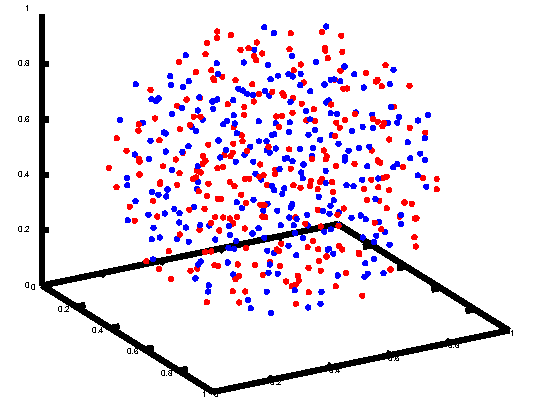
\includegraphics[width=0.5\textwidth]{figures/hball_500}
  \caption{Distribution \texttt{hammersley\_{}ball} with 500 randomly charged particles.}
\end{figure}

We choose the following parameter for our tests.

\begin{table}[p]
  \begin{footnotesize}
    \begin{center}
      \begin{tabular}{|r||c|c|c|c||c|c|c|c|}
        \hline \rule{0cm}{2.5ex}
        & \multicolumn{4}{c|}{FMM} & \multicolumn{4}{c|}{P2NFFT} \\
        \hline \rule{0cm}{2.5ex}
        N & ??? & ??? & ??? & ??? & $n$ & $m$ & $p$ & $\varepsilon_{I} = \varepsilon_{B}$ \\
        \hline
        500      & ??? & ??? & ??? & ??? & 32,32,32 & 2 & 5 & 3.5/32 \\
        5\,000   & ??? & ??? & ??? & ??? & 32,32,32 & 2 & 5 & 3.5/32 \\
        50\,000  & ??? & ??? & ??? & ??? & 64,64,64 & 2 & 5 & 3.5/64 \\
        500\,000 & ??? & ??? & ??? & ??? & 128,128,128 & 2 & 5 & 3.5/128 \\
        \hline
      \end{tabular}
    \end{center}
  \end{footnotesize}
  \caption{Parameters for the distribution \texttt{hammersley\_{}ball}}
\end{table}


\begin{table}[p]
  \centering
  \begin{tabular}{|r||r|r|r||c|c|}
    \hline
    $N$ & $t_\textrm{direct}$ & $t_\textrm{FMM}$ & $t_\textrm{P2NFFT}$ &
    \rule{0cm}{3ex}
    ${\cal E}^{\varphi}_{\mathrm rel}\left(\textrm{direct},\textrm{FMM}\right)$ &
    ${\cal E}^{\varphi}_{\mathrm rel}\left(\textrm{direct},\textrm{P2NFFT}\right)$ \\
    \hline
    500 & ??? & ??? & ??? & ??? & ??? \\
    5\,000 & ??? & ??? & ??? & ??? & ??? \\
    50\,000 & ??? & ??? & ??? & ??? & ??? \\
    500\,000& * & ??? & ??? & * & * \\
    \hline
  \end{tabular}
  \caption{Time and Error for 32 processes}
\end{table}

\begin{table}[p]
  \centering
  \begin{tabular}{|r||r|r||c|c|}
    \hline
    $P$ & $t_\textrm{FMM}$ & $t_\textrm{P2NFFT}$ &
    \rule{0cm}{3ex}
    ${\cal E}^{\varphi}_{\mathrm rel}\left(\textrm{ref},\textrm{FMM}\right)$ &
    ${\cal E}^{\varphi}_{\mathrm rel}\left(\textrm{ref},\textrm{P2NFFT}\right)$ \\
    \hline
    32   & ??? & ??? & ??? & ??? \\
    128  & ??? & ??? & ??? & ??? \\
    512  & ??? & ??? & ??? & ??? \\
    2048 & ??? & ??? & ??? & ??? \\
    8192 & ??? & ??? & ??? & ??? \\
    \hline
  \end{tabular}
  \caption{Strong scaling for $N=1\,000\,000$ particles and error bound ${\cal E}^{\varphi}_{\mathrm rel} \le 10^{-4}$}
\end{table}

\begin{table}[p]
  \centering
  \begin{tabular}{|r||r|r||c|c|}
    \hline
    $P$ & $t_\textrm{FMM}$ & $t_\textrm{P2NFFT}$ &
    \rule{0cm}{3ex}
    ${\cal E}^{\varphi}_{\mathrm rel}\left(\textrm{ref},\textrm{FMM}\right)$ &
    ${\cal E}^{\varphi}_{\mathrm rel}\left(\textrm{ref},\textrm{P2NFFT}\right)$ \\
    \hline
    32   & ??? & ??? & ??? & ??? \\
    128  & ??? & ??? & ??? & ??? \\
    512  & ??? & ??? & ??? & ??? \\
    2048 & ??? & ??? & ??? & ??? \\
    8192 & ??? & ??? & ??? & ??? \\
    \hline
  \end{tabular}
  \caption{Weak scaling for $N=1\,000\,000$ particles per process and error bound ${\cal E}^{\varphi}_{\mathrm rel} \le 10^{-4}$}
\end{table}

\subsection{Distribution \texttt{hammersley\_{}ball\_{}neg\_{}charge}}

As numerical test we used a ball uniformly filled with charged particles. The
total charge of the ball has been kept with $Q=-$1~nC. Thus the particles are assumed to
posses the charge $q_\ell=q=-1/N$~nC $(\ell=1,\dots,N)$, where $N$ denotes the number of
particles in the ball. These particles are also regarded as macro-particles representing
the distribution of all particles (for instance electrons) in a bunch. 

\begin{figure}[ht]
  \centering
  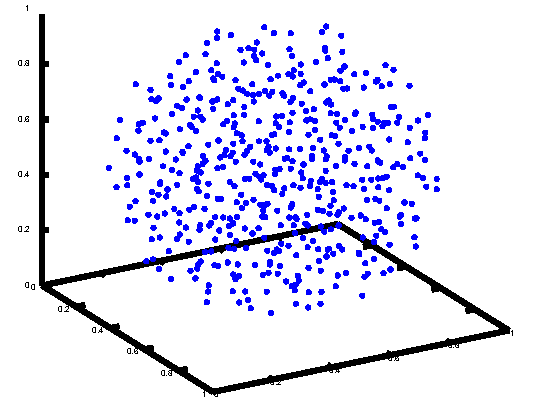
\includegraphics[width=0.5\textwidth]{figures/hballneg_500}
  \caption{Distribution \texttt{hammersley\_{}ball} with 500 negative charged particles.}
\end{figure}

Since a ball uniformly filled with an increasing number of particles
of equal charge gets more and more close to a ball with charge
$Q=\sum_{\ell=1}^N q_\ell$, we compare the results of the summation to
the analytically known potential of a homogeneously charged ball given
by (normalized by the factor $4\pi\varepsilon_0$)
% \[
%   \varphi_{\mbox {\tiny asym}}(\mathbf r_j)
%   = \frac{Q}{4\pi\varepsilon_0} \left(
%     \frac{3}{2}-\frac{\|\mathbf r_j\|}{2 R^2}\right)\, ,\qquad \|\mathbf r_j\|\leq R,
% \]
%% omit scaling with 1/(4*pi*eps0)
\[
  \varphi_{\mbox {\tiny asym}}(\mathbf r_j)
  = \frac{Q}{4\pi\varepsilon_0} \left(
    \frac{3}{2}-\frac{\|\mathbf r_j\|}{2 R^2}\right)\, ,\qquad \|\mathbf r_j\|\leq R,
\]
where $R$ denotes the radius of the ball.\par

\begin{table}[htb]
  \centering
  \begin{tabular}{|c||c|c|c|c|c|c|}
    \hline \rule{0mm}{5mm}
    $N$ & $t_{\mbox{\tiny slow}}$  &   $t_{\mbox{\tiny fast}}$
    &$\mathcal{E}_{\mathrm rel}^{\varphi}(\mbox{asym,slow})$
    &$\mathcal{E}_{\mathrm rel}^{\varphi}(\mbox{asym,P2NFFT})$
    &$\mathcal{E}_{\mathrm rel}^{\varphi}(\mbox{slow,P2NFFT})$  \\ \hline
    10\,000     & ??? & ??? & ??? & ??? &  ??? \\ \hline
    50\,000     & ??? & ??? & ??? & ??? &  ??? \\ \hline
    100\,000    & ??? & ??? & ??? & ??? &  ??? \\ \hline
    250\,000    & *   & ??? & *   & ??? &  *   \\ \hline
    500\,000    & *   & ??? & *   & ??? &  *   \\ \hline
    1\,000\,000 & *   & ??? & *   & ??? &  *   \\ \hline
  \end{tabular}
  \caption{Computational time and the error $\mathcal{E}_{\mathrm rel}$ for the potential $\varphi$, *estimated.\label{e2_potential}}
\end{table}
%
The numerical experiments documented in Table~\ref{e2_potential} show
that we obtain with our fast algorithm the same errors as with the
straightforward (slow) summation but with an numerical effort of only
$\mathcal{O}(N\log N)$. Hereby the parameters of the P2NFFT are chosen
such that the approximation error is less than the simulation error.
Finally, we test the algorithm for the computation of the
electrostatic field.  It is well known that the field of a
homogeneously charged ball is given by (normalized by the factor
$4\pi\varepsilon_0$)
% \[
% \mathbf E_{\mbox {\tiny asym}}(\mathbf r_j)
% =\frac{Q}{4\pi\varepsilon_0} \left( \frac{\mathbf r_j}{R^3}\right)\,
% ,\qquad \|\mathbf r_j\|\leq R.
% \]
%% omit scaling with 1/(4*pi*eps0)
\[
  \mathbf E_{\mbox {\tiny asym}}(\mathbf r_j)
  = Q \left( \frac{\mathbf r_j}{R^3}\right)\,,\qquad \|\mathbf r_j\|\leq R.
\]

% Table~\ref{e2_efield} represents the results of the related numerical simulations.
% Figure~\ref{nfft_times} compares the performance of P2NFFT to the direct slow summation.
% It shows that P2NFFT scales with $\mathcal{O}(N\log N)$.
% The numerical errors are acceptable (see Table~\ref{e2_potential}).
% Hence this new summation technique enables the computation of
% fully 3D particle-particle interactions in real life applications.


%%% Local Variables: 
%%% mode: latex
%%% TeX-master: ug.tex
%%% End: 




%% BIBTEX
\part{Bibliography}
\bibliographystyle{plainnat}
\bibliography{bibliography}

\part{Index}
\cleardoublepage
\pdfbookmark[0]{List of Tables}{lot}
\listoftables
\cleardoublepage
\pdfbookmark[0]{List of Figures}{lof}
\listoffigures
\cleardoublepage
%\pdfbookmark[-1]{Index}{index}
\printindex



\end{document}

%%% Local Variables: 
%%% mode: latex
%%% TeX-master: t
%%% End: 
